%\documentclass[11pt]{article}
\documentclass[11pt]{report}

\usepackage{amsmath, amstext, amssymb}
\usepackage{widetable}
\usepackage{booktabs}
\usepackage{newcent}
\usepackage{pstricks}
\usepackage{fancyhdr}
\usepackage[dvips]{graphicx}
\usepackage{makeidx}
\usepackage{psfrag}
\usepackage{alltt}
\usepackage{index}
\usepackage{fancyvrb}
\usepackage{pst-blur}
\usepackage{pst-grad}
\usepackage{epsfig}
%\usepackage{subfig}
\usepackage{subfigure}
\usepackage{xspace}
\usepackage{array}

\usepackage[colorlinks=true,linktocpage=true]{hyperref}

%% Listings package START
\usepackage{color}
\usepackage{listings}

\definecolor{darkblue}{rgb}{0,0,.6}
\definecolor{darkred}{rgb}{.6,0,0}
\definecolor{darkgreen}{rgb}{0,.6,0}
\definecolor{red}{rgb}{.98,0,0}
\definecolor{lightgrey}{rgb}{0.98,0.98,0.98}
\definecolor{black}{rgb}{0,0,0}

%\lstloadlanguages{C++}
%\lstset{
%  language=C++,
%  basicstyle=\small\ttfamily,
%  commentstyle=\itshape\color{darkgreen},
%  keywordstyle=\bfseries\color{darkblue},
%  stringstyle=\color{darkred},
%  showspaces=false,
%  showtabs=false,
%  columns=fixed,
%  backgroundcolor=\color{lightgrey},
%  numbers=none,
%  frame=single,
%  numberstyle=\tiny,
%  breaklines=true,
%  showstringspaces=false,
%  xleftmargin=0.1cm
%}
\lstset{
   language=C++,
   frame=lines,
   basicstyle=\small\ttfamily,
   keywordstyle=\bfseries\color{darkblue},
   stringstyle=\color{black}\ttfamily,
   tabsize=2,
   %emphstyle=\color{blue}\texttt
   commentstyle=\color{darkgreen}\ttfamily,
   numbers=left,
   numberstyle=\tiny,
   showstringspaces=false,
   literate={~} {$\sim$}{1}
}

\lstdefinelanguage{XML}
{
  morestring=[b]",
  morestring=[s]{>}{<},
  morecomment=[s]{<?}{?>},
  stringstyle=\color{black},
  identifierstyle=\color{darkblue},
  keywordstyle=\color{cyan},
  morekeywords={xmlns,version,type}% list your attributes here
}


\newcommand{\cmake}           {CMake\xspace}
\newcommand{\viennax}         {ViennaX\xspace}
\newcommand{\viennafactory}   {ViennaFactory\xspace}
\newcommand{\viennautils}     {ViennaUtils\xspace}
\newcommand{\gcc}             {GNU GCC\xspace}
\newcommand{\boost}           {Boost\xspace}
\newcommand{\plugin}          {plugin\xspace}
\newcommand{\openmpi}         {Open MPI\xspace}
\newcommand{\mpich}           {MPICH2\xspace}
\newcommand{\lammpi}          {LAM/MPI\xspace}

\renewcommand{\arraystretch}{1.2}


%\include{keywords}
\include{setup}

\begin{document}
\pagenumbering{roman}

% ==============================================================================
% TITLEPAGE
% ==============================================================================
\begin{titlepage}

\vspace*{3cm}
\Huge{ViennaWD}
\rule[0.0cm]{12.3cm}{0.05cm}
\begin{flushright}
\Large{User Manual\\}
\Large{v3.0.0}
%\Large{Building Instructions}\\
%\Large{Input Specifications}
\end{flushright}

\vspace{12cm}
\rule[0.0cm]{16.0cm}{0.05cm}
\begin{figure}[!ht]
   \vspace{-1.0cm}
   \centering
   \begin{minipage}{3cm}
      \epsfig{file=figures/TU_Signet_CMYK, scale=0.25}
   \end{minipage}
   \hfill
   \hspace{-0.5cm}
   \begin{minipage}{5.5cm}
      \vspace{0.5cm}
      \begin{center}
      Institute for Microelectronics\newline
      Technische Universit\"at Wien\newline
      Gu\ss hausstra\ss e 27-29 / E360\newline
      A-1040 Vienna, Austria\newline
      \end{center}
   \end{minipage}
   \hfill
   \begin{minipage}{2.6cm}
      \epsfig{file=figures/logo_px200, scale=1.6}
   \end{minipage}
\end{figure}

\end{titlepage}
% ==============================================================================
\clearpage
% ==============================================================================
% CONTRIBUTERS
% ==============================================================================
\begin{tabular}{ll}
Copyright {\copyright} 2012-2015 & Institute for Microelectronics, TU Wien.
\end{tabular}

\vspace{3.5cm}

\textbf{Principal Investigator:}\\
Mihail Nedjalkov\\

\textbf{Developers:}\\
Paul Ellinghaus\\
Josef Weinbub\\
Matthias Glanz\\

\textbf{Advisors:}\\
Ivan Dimov\\
Dragica Vasileska\\
Siegfried Selberherr\\

\textbf{Former Contributers:}\\
Marek Pobjecky\\
Philipp Schwaha\\



\vspace{7.0cm}

Institute for Microelectronics, TU Wien\newline
Gu\ss hausstra\ss e 27-29 / E360\newline
A-1040 Vienna, Austria/Europe\newline

\begin{tabular}{ll}
Phone  & +43-1-58801-36001\\
FAX    & +43-1-58801-36099\\
Web    & \texttt{http://www.iue.tuwien.ac.at/}
\end{tabular}

% ==============================================================================
%\addtocontents{toc}{\protect\setcounter{tocdepth}{1}}
\setcounter{tocdepth}{3}
\tableofcontents
\addcontentsline{toc}{chapter}{Contents}

\clearpage
\pagenumbering{arabic}


% ==============================================================================
\chapter{Overview}   %\addcontentsline{toc}{chapter}{Overview}
% ==============================================================================
ViennaWD is a suite of Monte Carlo simulation tools intended for the simulation of semiconductor devices in the classical domain and the investigation of quantum phenomena using the Wigner formalism. The suite encompasses the following simulation tools:
\begin{itemize}
  \item Wigner Ensemble Monte Carlo (WEMC)
  \item Classical Ensemble Monte Carlo (CEMC)
  \item Phonon Decoherence (PD)
\end{itemize}
The purpose, use and installation of each tool is discussed self-consistently in the following chapters.



\chapter{Building Information}

ViennaWD ships a central CMake~\cite{cmake} script, allowing to configure and build all simulators via one script.
In the following, we will discuss general installation aspects, however, for simulator-specific aspects please consult the respective
building-related sections.

\section{Build Configuration}

A default build configuration, which setup all simulators, is generated by:


\begin{lstlisting}
$> cd ViennaWD/
$> mkdir build
$> cd build
$> cmake ..
\end{lstlisting}


\NOTE{Watch for errors or warnings reported by CMake during the configuration process.}

\TIP{CMake will automatically try to discover the required dependencies on your system.}

\TIP{Use CMake's GUI application (\texttt{cmake-gui}) to conveniently select build features.}

\section{Configuration Options}

ViennaWD's build system allows to select the optimization level as well as the simulation tools to be generated by using the following CMake~\cite{cmake} options:

\begin{itemize}
  \item -D CMAKE\_BUILD\_TYPE=Debug$|$Release$|$RelWithDebInfo (default=Release)
  \item -D BUILD\_WEMC=OFF (default=ON)
  \item -D BUILD\_CEMC=ON (default=OFF)
  \item -D BUILD\_PD=ON (default=OFF)
\end{itemize}

\section{Building}

To build the simulators issue the following

\begin{lstlisting}
$> make
\end{lstlisting}

\TIP{Use \texttt{-jN}, where \texttt{N} refers to the number of parallel jobs/available CPU cores, to speed-up the build process.}


% ==============================================================================
% Add Project specifc external Latex source file
% ==============================================================================

% ==============================================================================
\chapter{Wigner Ensemble Monte Carlo}   %\addcontentsline{toc}{chapter}{Introduction} \label{intro}
% ==============================================================================

\section{Introduction}
Wigner Ensemble Monte Carlo (WEMC) is a C-based simulator, with MPI parallelisation, for quantum transport simulations in one- and two-dimensional structures.

The Wigner formalism expresses quantum mechanics in terms of functions and variables in the phase space. Such a formulation allows a more intuitive insight, versus wave functions and operators, and allows the utilization of some classical notions, e.g. Boltzmann scattering. The Wigner function is known as a quasi-distribution function since, despite negative values occurring, it can be used in the same way as a true distribution function to calculate physical averages of interest, e.g. density or current. The Wigner equation describes the temporal evolution of the Wigner function, $f_w$. The choice of a finite coherence length $L$ \cite{signParticle2D} yields the semi-discrete form of the Wigner equation, the one-dimensional version of which is defined as
\begin{equation}
\frac{\partial f_{w}}{\partial t}+\frac{\hbar q\Delta k}{m^{*}}\frac{\partial f_{w}}{\partial x}={\displaystyle \sum_{q=-K}^{K}V_{w}\left(x,q-q',t\right)f_{w}\left(x,q',t\right)},\label{eq:semi-discrete-wigner-eq}
\end{equation}
where $q$ is an index which represents the quantized momentum, i.e. $p=\hbar\left(q\Delta k\right)$. The resolution $\Delta k$ is determined by the coherence length, $\Delta k=\frac{\pi}{L}$. The effective mass is represented by $m^*$ in the above equation. The Wigner potential $V_w$ is defined as
\begin{eqnarray}
V_{w}\left(x,q\right) & \equiv & \frac{1}{i\hbar L}\int_{-\frac{L}{2}}^{\frac{L}{2}}ds\, e^{-i2q\Delta k\cdot s}\delta V\left(s;x\right);\label{eq:semi-discrete-wigner-potential}\\
\delta V\left(s;x\right) & \equiv & V\left(x+s\right)-V\left(x-s\right).\nonumber
\end{eqnarray}

The WEMC simulator solves (\ref{eq:semi-discrete-wigner-eq}), using the signed-particle Monte Carlo method \cite{Mixi_MCmethod_APL} for the one- and two-dimensional case. The evolution of an initial condition, e.g. a minimum uncertainty wave packet (default), can be investigated in the presence of a static potential profile. The minimum uncertainty wave packet is defined as
\begin{equation}
\psi\left(x,t_{0}\right)=\left(2\pi\sigma^{2}\right)^{-\frac{1}{4}}e^{-\frac{\left(x-x_{0}\right)^{2}}{4\sigma^{2}}}e^{ik_{0}z},\label{eq:initial_condition}
\end{equation}
where $\sigma$, $x_0$ and $k_0$ represent the standard deviation (in space), the mean position and the mean momentum (i.t.o. $k$), respectively. The initial condition and the potential profile can be specified using input files (discussed in Section~\ref{ch:simulations}). 

Boltzmann-type scattering mechanisms can be selectively activated. Currently, models for acoustic, Coulomb, optical (intravalley), XX/LL/XL intervalley and surface roughness are implemented for the silicon material system.

The simulator offers parallel execution in a distributed-memory environment, using MPI. The parallelization approach is based on a spatial domain decomposition where each MPI process is assigned a part of the domain and treats only particles present in its subdomain. Further details can be found in \cite{JCEL_MPI}\cite{JCEL_MPI_2}.



% ==============================================================================
% ==============================================================================
\section{Building Information} %\addcontentsline{toc}{chapter}{Building Instructions} \label{building}
% ==============================================================================
% ==============================================================================

\subsection{Dependencies}

The following list represents the required packages to build and execute the WEMC simulator.
Note that a serial version and a parallel MPI version of the simulator can be compiled,
requiring an appropriate MPI library.


\begin{itemize}
  \item C-Compiler (e.g. GCC~\cite{gcc} Version $\geq4.4$)
  \item CMake~\cite{cmake} Version $\geq2.6$
  \item GSL~\cite{gsl} Version $\geq1.16$
  \item FFTW~\cite{fftw} Version $\geq3.3.3$
  \item Lua~\cite{lua} Version $5.1$
  \item MPI (e.g. OpenMPI~\cite{openmpi} Version $\geq1.3$) - optional -
%  \item OpenMP~\cite{openmp} Version $\geq3.0$ - optional -
  \item gnuplot	\cite{gnuplot} Version $\geq4.2$ - optional -
  \item Python \cite{python} Version $\geq3.0$ - optional -
\end{itemize}

\TIP{All external dependencies are usually shipped with the popular Linux distributions.
For instance, on Linux Mint check for the following packages to install the aforementioned packages: cmake, libgsl0-dev, libfftw3-dev, liblua5.1-0-dev, openmpi-bin}

\subsection{Configuration Options}


Several optional configuration targets are provided, such as:

\begin{itemize}
  \item -D USE\_MPI=OFF (default=ON)
%  \item -D USE\_OPENMP=ON (default=OFF)
  \item -D DEBUG\_OUTPUT=OFF (default=ON)
  \item -D FILE\_OUTPUT=OFF (default=ON)
  \item -D BUILD\_TESTS=OFF (default=ON)
\end{itemize}

To build only the serial version of the simulator the following configuration can be used, for instance:

\begin{lstlisting}
$> cmake -D USE_MPI=OFF ..
\end{lstlisting}

To build the parallel MPI version of the simulator in addition to the serial version, use the following configuration:

\begin{lstlisting}
$> cmake -D USE_MPI=ON ..
\end{lstlisting}




% ==============================================================================
% ==============================================================================
\section{Simulations} \label{ch:simulations} %\addcontentsline{toc}{chapter}{Building Instructions} \label{building}
% ==============================================================================
% ==============================================================================

\subsection{Simulator Control}

The simulations are set up via text-based configuration file, which allows the user to specify various parameters. Furthermore, there exists the option to specify a potential profile and/or an initial state and/or a working directory where output files of the simulator are saved. The details of these input files/arguments are discussed in the following.

\subsubsection{Configuration}

The simulation parameters that can be specified by the user are fed to the simulator using a text-based Lua~\cite{lua} input file. The parameters pertain to a specification of the simulation domain, computational aspects and physical models (amongst other things). The configuration file \texttt{examples/full\_config.lua} explains all user-specifiable parameters along with their default values. Only certain parameters must be specified; optional parameters revert to default values if not specified. %Table \ref{tab:lua-params} lists all parameters, with their meaning, default values (if applicable) and valid ranges.

The simulation domain is defined by specifying the minimum and maximum values along each axis, i.e. the boundaries of a rectangle. A one-dimensional domain must be specified using the $y$ parameters;  the $x$-values must be set to zero. Two kinds of boundary conditions can be specified, namely absorbing or reflecting, for each of the four boundaries (two in 1D case).

%The parameters of (\ref{eq:wave-packet}) appearing in \ref{tab:lua-params} can be specified in the lua file. The square potential barrier is defined through the position of its left edge, its width and height, as specified in \ref{tab:lua-params}. Note that due to the finite mesh-size value, the rectangular is represented as a trapezium.
%Parameters that do not appear in the table should be left unaltered.

%\clearpage

%\begin{table}[ht]
%\caption{Input parameters for Lua file\label{tab:lua-params} }
%\begin{widetable}{\columnwidth}{ccl}
%\toprule
%Parameter name & Units & Remark\\
%\midrule
%\texttt{x0, y0} & m & mean position of wave packet\\
%\texttt{sigmaX, sigmaY} & m & spatial standard deviation\\
%\texttt{k0x, k0y} & 1 & mean momentum offset $(\texttt{k0}\, \hbar\Delta k)$ \\
%\midrule
%\texttt{barrier\_left\_edge} & m & start position of barrier\\
%\texttt{barrier\_width} & m & width of barrier\\
%\texttt{V1} & eV & height of potential barrier\\
%\midrule
%\texttt{mesh\_size} & m & spacing between mesh nodes (uniform)\\
%\texttt{L\_coh} & m & coherence length\\
%\midrule
%\texttt{Lx1/2} & m & minimum/maximum of domain in x-direction\\
%\texttt{Ly1/2} & m & minimum/maximum of domain in y-direction\\
%\texttt{BC1/2/3/4} & - & boundary condition at Lx1/2, Ly1/2\\
%\midrule
%\texttt{global_max_particles} & 1 & maximum number of parti\\
%\texttt{dt} & s & time step (where annihilation can be performed)\\
%\texttt{total\_time} & s & total simulation time\\
%\texttt{signed\_total} & 1 & number of particles initialized in wave packet\\

%\bottomrule
%\end{widetable}
%\end{table}

Other examples of configuration files are shipped with WEMC and are located under

\begin{lstlisting}
wigner_ensemble_monte_carlo/examples/
\end{lstlisting}

The configuration file is passed to the simulator as the first argument. For the serial simulator this can be done by

\begin{lstlisting}
$> cd ViennaWD/build/wigner_ensemble_monte_carlo/
$> ./wemcsim ../../wigner_ensemble_monte_carlo/examples/configuration.lua
\end{lstlisting}

or, when using the MPI-enabled simulator, by

\begin{lstlisting}
$> cd ViennaWD/build/wigner_ensemble_monte_carlo/
$> mpirun -np 4 ./wemcsim_mpi \
   ../../wigner_ensemble_monte_carlo/examples/configuration.lua
\end{lstlisting}

\subsubsection{Potential profile}

The default potential profile is a square potential barrier of which the parameters can be specified in the Lua configuration file; if no parameters are specified in the configuration file a constant (zero) potential is assumed. The potential profile is hard-coded in the file \linebreak \texttt{src/potential\_profile.c}. This file contains several parameterized analytical formulas in functions, which can be extended and combined to construct a potential profile. Otherwise, the simulator also offers the possibility to specify a potential profile using a CSV file.
%A time-dependent potential profile can also be specified, but is currently only supported in the serial version of the simulator. 

The filename of the potential profile must contain the string "potential" to be correctly identified as a potential input for the simulator, e.g. \texttt{potential\_profile\_example.csv}. Currently, the simulator only supports a uniform rectangular mesh. The user must ensure that the grid specified in the potential profile matches the dimensions and mesh size specified in the Lua input file. The profile is saved in a simple CSV format: the x-position~[m], y-position~[m] and potential~[eV] are specified, using a space as a delimiter between them; each x-value is associated with a block of y-values. The file for a one-dimensional profile should contain an x-value of zero in the first column. For an example, refer to the files \texttt{examples/potential\_*\_example*.csv}. 

The execution of the simulator with the specification of a potential profile in a CSV file is done as follows:
\begin{lstlisting}
$> cd ViennaWD/build/wigner_ensemble_monte_carlo/
$> ./wemcsim ../../wigner_ensemble_monte_carlo/examples/configuration.lua \
   /dir_with_potential_files/potential_example.csv
\end{lstlisting}


\subsubsection{Initial condition}

The default initial condition, which can be specified in the Lua configuration file, is a single minimum uncertainty wave packet, as defined in (\ref{eq:initial_condition}) (and its 2D analogue). 
If a different initial condition is desired, the file \texttt{src/particle\_initialization.c} can be modified. Alternatively, the initial condition can be specified by an input file. The initial condition can be specified using either a Wigner function or a particle ensemble. 

The Wigner function is specified in a file by defining its value for each cell in the phase space. The values of the Wigner function can be negative, however, the sum of all values should still add up to 1. The absolute value of the Wigner function in each cell is multiplied by the value of \texttt{signed\_total}, specified in the configuration file, and the resulting number of particles are generated in the cell with a sign corresponding to that of the Wigner function. The size of the phase space cells specified in the file must be compatible with the dimensions, mesh size and coherence length specified in the configuration file. The filename of the Wigner function must be named as \texttt{*wigner*.csv}, where the string "wigner" is used to correctly identify the file as an input for the initial condition in the form of a Wigner function. 

The initial condition can also be specified through an input file defining the ensemble of particles with the properties of each particle. This method of specifying the initial condition is intended to start the simulator from a state simulated before and saved to file using the function \texttt{saveParticleStack()} in the the file \texttt{save\_funcs.c}. In principle, the particle ensemble can also be generated otherwise (with all the required properties for each particle) and imported by the simulator. The simulator reads the input file using the function \texttt{readParticleStack()} in the file \texttt{particle\_initialization.c}. The filename of the particle ensemble must be named as \texttt{*particle*.csv}, where the string "particle" is used to correctly identify the file as an input for the initial condition in the form of a particle ensemble.

\TIP{The total number of initialized particles should not exceed the global maximum specified in the configuration file. A total of at most half the maximum value is advisable to accommodate particle generation using reasonable time steps.}

The execution of the simulator with the specification of an initial condition in the form of a Wigner function in a CSV file is done as follows:
\begin{lstlisting}
$> cd ViennaWD/build/wigner_ensemble_monte_carlo/
$> ./wemcsim ../../wigner_ensemble_monte_carlo/examples/configuration.lua \
   /dir_with_initial_conditions/wigner_IC_example.csv
\end{lstlisting}
Similarly, the MPI-enabled version can be called; an example where both a potential profile and an initial condition in the form of a particle ensemble is specified is done as follows:
\begin{lstlisting}
$> cd ViennaWD/build/wigner_ensemble_monte_carlo/
$> mpirun -np 4 ./wemcsim_mpi \
   ../../wigner_ensemble_monte_carlo/examples/configuration.lua \
   /dir_with_initial_conditions/particle_ensemble_IC_example.csv \
   /dir_with_potentials/potential_example.csv
\end{lstlisting}


\subsubsection{Working directory}
The directory where files, containing the physical quantities specified in the Lua file, are saved can be specified by an additional argument:

\begin{lstlisting}
$> mkdir ~/work_dir
$> cd ViennaWD/build/wigner_ensemble_monte_carlo/
$> mpirun -np 4 ./wemcsim_mpi \
   ../../wigner_ensemble_monte_carlo/examples/configuration.lua ~/work_dir
\end{lstlisting}

If no directory is specified, the default directory used is \texttt{/tmp/}.

\subsection{Output}

The WEMC simulator can calculate various physical quantities and distributions, which are saved in the working directory with a time stamp, using the file names and functions specified in Table~\ref{tab:save-funcs}. The associated functions can be found in \texttt{src/save\_funcs.c} and are summoned at the specified save interval in the function \texttt{saveData()}. In the case of a parallel execution with MPI, the quantities associated to the subdomain of each process are saved and must be merged by a post-processing script (see Section~\ref{sec:post-proc}).

The quantities are represented in the spatial and/or $k$ domain(s) as histograms and follow a similar template: the range of the bins (i.e. minimum (inclusive) and maximum (exclusive) value) is followed by the probability of finding a particle within the stated range of the bin(s). Negative values may arise  for 'probabilities' of (partial) Wigner distributions or in physical quantities due to numerical approximations/noise made when solving the Wigner equation. 
%The quantities can be automatically plotted using the provided plotting scripts (for gnuplot). 
%\begin{lstlisting}
%$> cd build
%$> gnuplot
%gnuplot> plot 'density_t20.csv' u 3:5 with lines
%\end{lstlisting}

%\TIP{Very small negative values for probabilities may arise due to \linebreak numerical approximations that are made in solving the Wigner equation}


\NOTE{ The particle stack and Wigner function result in very large file size(s) and should not be saved regularly to avoid excessive file I/O. }

\begin{table}[h]
\caption{Simulator output\label{tab:save-funcs} }
\begin{widetable}{\columnwidth}{lll}
\toprule
Data & File name & Function\\
\midrule
Spatial distribution & density\_t*.csv & \texttt{saveDensity()}\\
Momentum distribution & Kdistrib\_t*.csv & \texttt{saveKdistrib()} \\
Particle stack & particleStack\_t*.csv & \texttt{saveParticleStack()}\\
Wigner function & wignerFunciton\_t*.csv & \texttt{saveWignerFunction()}\\
Potential profile & potential\_profile\_t*.csv & \texttt{savePotential()}\\
Particle generation rate & gamma.csv & \texttt{saveGamma()}\\
Energy distribution & energy\_t*.csv & \texttt{saveEnergyDistrib()}\\
Current & current.csv & \texttt{saveCurrent()}\\
Density distribution f(x,kx) & x\_kx\_t*.csv & \texttt{saveXDensK()}\\
Density distribution f(y,ky) & y\_ky\_t*.csv & \texttt{saveYDensK()}\\
\bottomrule
\end{widetable}
\end{table}


\subsection{Post-processing}\label{sec:post-proc}

After the simulator has completed its simulation the generated data needs to be merged (in the case of parallel execution) and (optionally) plots of the data can be generated. The quantities to be saved/merged and (optionally) plotted are specified by flags, e.g. save\_density, in the Lua input file. There are three possible values for each flag, explained in Table~\ref{tab:save-flag-ops}.
\begin{table}[!h]
\caption{Save flag options\label{tab:save-flag-ops} }
\begin{widetable}{\columnwidth}{lll}
\toprule
Flag value & Meaning\\
\midrule
0 & no output data generated by the simulator\\
1 & calculate and save quantity; merged by post\_processing.py\\
2 & calculate and save quantity; merged and plotted by post\_processing.py\\
\bottomrule
\end{widetable}
\end{table}
 
The Python script \texttt{tools/post\_processing.py} performs the merging and plotting tasks by reading the simulation setup file, \texttt{SimulationSetup.txt}. This file is generated by the simulator during execution in \texttt{work\_dir} and contains the values of the flags in the original input file and other information, e.g. the number of MPI processes, which are acquired at run-time. After the simulator (\texttt{wemcsim} or \texttt{wemcsim\_mpi}) is finished the script \texttt{tools/post\_processing.py} must be called manually; the working directory \texttt{work\_dir}, which contains the generated output data, must be specified as an argument:
\begin{lstlisting}
$> cd ViennaWD/wigner_ensemble_monte_carlo/tools/
$> python post_processing.py /work_dir/
\end{lstlisting}
In case of a parallel execution with \texttt{wemcsim\_mpi}, the script merges the data files (prepended by a 'p' e.g. \texttt{p*\_density\_t*.csv} ) generated by the MPI processes into one file, which  represents the global domain, and then deletes the files associated with the sub-domains. The script saves the merged CSV files in the working directory (referred to as \texttt{work\_dir}). 

After merging the data files, plots are generated for the quantities specified with a flag value of 2 and can be found in the folder \texttt{work\_dir/results}. The post-processing script prepares the data files (if needed) and calls the gnuplot scripts in \texttt{/plot\_scripts}. The plots are saved as images in the GIF file format, which requires the gif terminal to be available in gnuplot. The terminals installed for gnuplot can be checked as follows:
\begin{lstlisting}
$> gnuplot
$> set terminal
$> Available terminal types:
$>           canvas  HTML Canvas object
$>              cgm  Computer Graphics Metafile
$>         epscairo  eps terminal based on cairo

\end{lstlisting}
If \texttt{gif} is not listed, the package \texttt{libgd2-dev} should be installed. This library also provides the jpeg and png functionality of gnuplot. Alternatively, the file format for the generated plots can be changed manually in the gnuplot scripts in \texttt{/plot\_scripts/} from gif to another terminal type.
%Scripts for the visualization of quantities using gnuplot and/or Paraview are provided in the directory \texttt{plot\_scripts/}, but still require manual modifications of axes scales, file names etc.

All merging and plotting can still be done be performed individually by manually calling the various plot and merge scripts, which \texttt{post\_processing.py} does automatically.
\clearpage
% ==============================================================================
% ==============================================================================
\section{License}  %\addcontentsline{toc}{chapter}{Appendix A: License}

Copyright (c) 2013-2015, Institute for Microelectronics, TU Wien

Permission is hereby granted, free of charge, to any person obtaining a copy
of this software and associated documentation files (the "Software"), to deal
in the Software without restriction, including without limitation the rights
to use, copy, modify, merge, publish, distribute, sublicense, and/or sell
copies of the Software, and to permit persons to whom the Software is
furnished to do so, subject to the following conditions:

The above copyright notice and this permission notice shall be included in
all copies or substantial portions of the Software.

THE SOFTWARE IS PROVIDED "AS IS", WITHOUT WARRANTY OF ANY KIND, EXPRESS OR
IMPLIED, INCLUDING BUT NOT LIMITED TO THE WARRANTIES OF MERCHANTABILITY,
FITNESS FOR A PARTICULAR PURPOSE AND NONINFRINGEMENT. IN NO EVENT SHALL THE
AUTHORS OR COPYRIGHT HOLDERS BE LIABLE FOR ANY CLAIM, DAMAGES OR OTHER
LIABILITY, WHETHER IN AN ACTION OF CONTRACT, TORT OR OTHERWISE, ARISING FROM,
OUT OF OR IN CONNECTION WITH THE SOFTWARE OR THE USE OR OTHER DEALINGS IN
THE SOFTWARE.
% ==============================================================================
% ==============================================================================


% ==============================================================================
\chapter{Classic Ensemble Monte Carlo}   \label{emc}
% ==============================================================================

\section{Introduction}
The Classic Ensemble Monte Carlo (CEMC) tool is designed for simulating two-dimensional MOSFET devices by means of solving the Boltzmann transport
equation using the Ensemble Monte Carlo algorithm. It is based on Fortran code developed
by Prof. Dragica Vasileska from Arizona State University. The original Fortran code has been translated to C and optimized.

Currently the implemented scattering mechanism include Coulomb scattering (Brooks-Herring approach),
acoustic phonon scattering and intervalley scattering (zero-order f and g absorption and emission processes).
The implemented 2D Monte Carlo Poisson solver solves the 2D Poisson-equation using the successive over-relaxation (SOR) method.

%% ==============================================================================
%% ==============================================================================
%\section{Building Instructions} \label{boltzmann:building}
%% ==============================================================================
%% ==============================================================================

%The CEMC simulator is generated by the central ViennaWD CMake build system.

%\begin{lstlisting}
%$> cd ViennaWD/
%$>
%\end{lstlisting}

%The Makefile compiles the source files with the command

%\begin{lstlisting}
%$> gcc -c -Wall -O3 -g3 -pedantic
%\end{lstlisting}

%and creates an executable \texttt{viennaemc} which can be simply executed by typing

%\begin{lstlisting}
%$> ./viennaemc
%\end{lstlisting}

%\TIP{The input files which need to be in the same directory as the executable are read automatically.}

%To remove the executable and object files type
%\begin{lstlisting}
%$> make clean
%\end{lstlisting}

% ==============================================================================
% ==============================================================================
\section{Building Information} %\addcontentsline{toc}{chapter}{Building Instructions} \label{building}
% ==============================================================================
% ==============================================================================

% ==============================================================================
\subsection{Dependencies} \label{boltzmann:dependencies}
% ==============================================================================
%The CEMC tool depends on the math library (\texttt{libm}), which is available on all Unix systems and automatically
%discovered and linked by the CMake build system.

In the following the dependencies of the CEMC simulator are presented.

\begin{itemize}
  \item C-Compiler (e.g. GCC~\cite{gcc} Version $\geq4.4$)
  \item Math library (Unix Standard)
\end{itemize}

%The ViennaEMC library uses only standard \textit{C} libraries and does not depend on any external libraries.
%Only a suitable C compiler (e.g. GCC) is necessary.


% ==============================================================================
\section{Examples} \label{boltzmann:examples}
% ==============================================================================
Three examples are shipped with this package.

The first example can be found in the directory

\texttt{examples/example01}

and contains input files with default values as described in Section~\ref{boltzmann:sim},
Table~\ref{tab:simpar} and Table~\ref{tab:devdim} (MOSFET device in on-state).

The second example is located in the directory

\texttt{examples/example02}

and contains the same device geometry with zero drain voltage (\texttt{inputVd = 0.0}) representing a MOSFET device in off-state.


The first two examples can be executed by the following.
\begin{lstlisting}
$> cd ViennaWD/build/classic_ensemble_monte_carlo/
$> ./emc ../../classic_ensemble_monte_carlo/examples/example0x/device_dimensions.in
     ../../classic_ensemble_monte_carlo/examples/example0x/simulation_parameters.in
\end{lstlisting}

The third example is located in the directory

\texttt{examples/example03}

and contains an example of how to use the simulator kernel in an external C++ program. The example consists of a \texttt{main.cpp} C++ source code file where a minimalist code required to run the simulator is given.
The following data structures
\begin{itemize}
\item \texttt{const\_t constants;}
\item \texttt{geometry\_t *geometry;}
\item \texttt{scatpar\_t *scatpar;}
\item \texttt{phys\_quant\_t *phys\_quantities;}
\item \texttt{output\_t *outputdata;}
\end{itemize}
must be declared and allocated as shown. Then the user needs to initialize the simulation parameters shown in table \ref{tab:simpar} as well as the device dimension parameters shown in table \ref{tab:devdim}. Also the following initialization functions
\begin{itemize}
\item \texttt{oooMatParInitialization(\&constants);}
\item \texttt{oooScatParInitialization(scatpar);}
\item \texttt{oooDeviceStructureInitialization(constants, geometry, scatpar);}
\end{itemize}
must be called as shown to initialize the data structures. \\
The simulator itself is started by calling: \\
\texttt{outputdata = EMC(constants, geometry, scatpar, phys\_quantities);} \\
This function has a return value of type \texttt{output\_t *} and returns a pointer to the output data which can be processed in the next step. The output data structure is described in section \ref{boltzmann:out}. Finally the allocated memory needs to be freed in order to avoid memory leaks before exiting the program.

%\TIP{Keep the default parameters described in Section \ref{boltzmann:sim}, tables \ref{tab:mc2d}, \ref{tab:matpar}, \ref{tab:scatflag} and \ref{tab:scatpar} when compiling an executable for running the examples. Alternatively all source files and the Makefile can be copied to the corresponding example folder and compiled there using \texttt{make}.}

% ==============================================================================
% ==============================================================================
\section{Simulation Control} \label{boltzmann:sim}
% ==============================================================================
% ==============================================================================

The simulations can be controlled by two input files:
\begin{itemize}
\item \texttt{simulation\_parameters.in}
\item \texttt{device\_dimensions.in},
\end{itemize}
which are read in the main program as well as constants defined in \texttt{emc.h} and silicon material parameters implemented in \texttt{mat\_par\_initialization.c}
located in the \texttt{src} folder.
This section describes all relevant parameters.

\subsection{Input file format}

Simulation parameters contained in \texttt{simulation\_parameters.in} are described in table \ref{tab:simpar}.

\begin{table}[ht!]
\centering
\begin{tabular}{|l|p{7cm}|c|c|}
\hline
\textbf{Variable}                    &  \textbf{Definition}                           &  \textbf{Default} \\
\hline
\texttt{scatpar->dt}                 &  differential time step in $[s]$               &  $1.5e^{-16}$ \\
\hline
\texttt{scatpar->totalTime}          &  total time to be simulated in $[s]$           &  $10e^{-12}$ \\
\hline
\texttt{scatpar->transientTime}      &  duration of the initial transient in $[s]$    &  $3.0e^{-12}$ \\
\hline
\texttt{scatpar->averTime}           &  averaging time in $[s]$                       &  $2.0e^{-13}$ \\
\hline
\texttt{phys\_quantities->inputVs}   &  input source voltage in $[V]$                 &  $0.0$ \\
\hline
\texttt{phys\_quantities->inputVd}   &  input drain voltage in $[V]$                  &  $1.0$\\
\hline
\texttt{phys\_quantities->inputVg}   &  input gate voltage in $[V]$                   &  $1.0$ \\
\hline
\texttt{phys\_quantities->inputVsub} &  input substrate voltage in $[V]$              &  $0.0$\\
\hline
\texttt{constants.omega}             &  relaxation factor for the SOR Poisson solver, should be in the range $1 \leq \omega \leq 2$  &  $1.8$ \\
\hline
\texttt{constants.tolerance}         &  convergence tolerance for the Poisson solver  &  $1e^{-4}$\\
\hline
\end{tabular}
\caption{The input variables in \texttt{simulaton\_parameters.in} are described.}
\label{tab:simpar}
\end{table}

The device parameters contained in \texttt{device\_dimensions.in} are described in table \ref{tab:devdim}.

\begin{table}[ht!]
\centering
\begin{tabular}{|l|p{8.0cm}|c|c|}
\hline
\textbf{Variable}                 &  \textbf{Definition}                              &  \textbf{Default} \\
\hline
\texttt{geometry->lengthSD}       &  length of the source and drain contacts in $[m]$ &  $50e^{-9}$ \\
\hline
\texttt{geometry->depthSD}        &  depth of the source and drain contacts in $[m]$  &  $30e^{-9}$ \\
\hline
\texttt{geometry->lengthG}        &  length of the gate in $[m]$                      &  $25e^{-9}$ \\
\hline
\texttt{geometry->depthB}         &  bulk depth in $[m]$                              &  $70e^{-9}$ \\
\hline
\texttt{geometry->deviceWidth}    &  width of the device in $[m]$                     &  $1e^{-6}$ \\
\hline
\texttt{geometry->oxideThickness} &  thickness of the $SiO_2$ layer in $[m]$          &  $1.2e^{-9}$\\
\hline
\texttt{geometry->meshSize}       &  mesh size in $[m]$                               &  $1e^{-9}$ \\
\hline
\texttt{scatpar->dopingCon{[0]}}  &  doping concentration for region 1 in $[m^{-3}]$  &  $5e^{25}$\\
\hline
\texttt{scatpar->dopingCon{[1]}}  &  doping concentration for region 2 in $[m^{-3}]$  &  $5e^{25}$ \\
\hline
\texttt{scatpar->dopingCon{[2]}}  &  doping concentration for region 3 in $[m^{-3}]$  &  $-5e^{24}$\\
\hline
\texttt{scatpar->dopingCon{[3]}}  &  doping concentration for region 4 in $[m^{-3}]$  &  $-5e^{23}$\\
\hline
\end{tabular}
\caption{The input variables in \texttt{device\_dimensions.in} are described.}
\label{tab:devdim}
\end{table}



\subsection{\texttt{emc.h} header file description}

The \texttt{emc.h} header file contains constant definitions as well as data structure and function declarations.
Relevant macros are depicted in Table~\ref{tab:emc}.

\clearpage

\begin{table}[ht!]
\centering
\begin{tabular}{|l|p{9cm}|c|c|}
\hline
\textbf{Constant}        & \textbf{Definition}                               & \textbf{Default} \\
\hline
\texttt{\#define MAXNX}  & maximum mesh x coordinate                         &  $200$ \\
\hline
\texttt{\#define MAXNY}  & maximum mesh y coordinate                         &  $200$ \\
\hline
\texttt{\#define DOPREG} & maximum number of doping regions                  &  $4$ \\
\hline
\texttt{\#define MAXSC}  & maximum number of scattering mechanisms           &  $10$ \\
\hline
\texttt{\#define NLEV}   &  number of energy levels in the scattering table  &  $1000$ \\
\hline
\texttt{\#define MAXEN}  &  maximum number of electrons                      &  $1000000$\\
\hline
\end{tabular}
\caption{The constant definitions in \texttt{emc.h} are shown.}
\label{tab:emc}
\end{table}

\TIP{The user may need to modify the constants \texttt{MAXNX} and \texttt{MAXNY} if the default values exceed the ratios $\frac{device \: x-length}{mesh \: size}$ and $\frac{device \: y-length}{mesh \: size}$.}

\TIP{\texttt{MAXEN} may also be modified by the user in case the simulator reports the error \textit{Actual number of electrons exceeds \texttt{MAXEN}}.}


\subsection{Material \& Scattering parameters}

The material parameters for Silicon are defined in \texttt{mat\_par\_initialization.c}. The table \ref{tab:matpar} shows material parameter variables that may be modified by the user if needed.

\begin{table}[ht!]
\centering
\begin{tabular}{|l|l|c|}
\hline
\textbf{Variable}             & \textbf{Definition}                       & \textbf{Default value} \\
\hline
\texttt{TL}                   & lattice temperature in $[K]$              & $300.0$ \\
\hline
\texttt{am\_l}                & lateral effective mass                    & $0.91$ \\
\hline
\texttt{am\_t}                & transversal effective mass                & $0.19$ \\
\hline
\texttt{constpar->eps\_sc}    & relative permittivity of Silicon          & $11.8 \: \varepsilon_0$\\
\hline
\texttt{constpar->eps\_ox}    & relative permittivity of $SiO_{2}$        & $3.9 \: \varepsilon_0$\\
\hline
\texttt{constpar->Ni}         & intrinsic carrier density in Silicon      & $1.45e^{16}$ \\
\hline
\texttt{constpar->delta\_Ec}  & half band gap energy normalized by $V_T$  & $0.575 / \texttt{constpar->vt}$ \\
\hline
\texttt{constpar->density}    & Silicon density in $[kg/m^{3}]$           & $2329.0$ \\
\hline
\texttt{scatpar->vsound}      & sound velocity in Silicon in $[m/s]$      & $9040.0$ \\
\hline
\texttt{constpar->af}         & non-parabolicity factor                   & $0.5$ \\
\hline
\end{tabular}
\caption{User modifiable material parameters and their respective default values in \texttt{mat\_par\_initialization.c} are shown.}
\label{tab:matpar}
\end{table}

Scattering mechanisms are controlled by setting the variable switches listed in table \ref{tab:scatflag}.

\TIP{By default, coulomb scattering, acoustic phonon scattering and intervalley zero-order scattering are enabled whereas intervalley first-order scattering and surface roughness are disabled.}

\begin{table}[ht!]
\centering
\begin{tabular}{|l|p{5cm}|c|}
\hline
\textbf{Variable}                    & \textbf{Mechanism}                                  & \textbf{Value} \\
\hline
\texttt{scatpar->coulombscattering}  & coulomb scattering                                  & 0 .. off, 1 .. on \\
\hline
\texttt{scatpar->acousticscattering} & acoustic phonon scattering                          & 0 .. off, 1 .. on \\
\hline
\texttt{scatpar->intervalley0g}      & intervalley phonon scattering zero order g-process  & 0 .. off, 1 .. on \\
\hline
\texttt{scatpar->intervalley0f}      & intervalley phonon scattering zero order f-process  & 0 .. off, 1 .. on \\
\hline
\texttt{scatpar->intervalley1g}      & intervalley phonon scattering first order g-process & 0 .. off, 1 .. on \\
\hline
\texttt{scatpar->intervalley1f}      & intervalley phonon scattering first order f-process & 0 .. off, 1 .. on \\
\hline
\texttt{scatpar->surfaceroughness}   & surface roughness                                   & 0 .. off, 1 .. on \\
\hline
\end{tabular}
\caption{Scattering mechanism selection variables \texttt{mat\_par\_initialization.c} are shown.}
\label{tab:scatflag}
\end{table}

Parameters for the scattering processes can be modified by setting the corresponding variables listed in table \ref{tab:scatpar}.

\begin{table}[ht!]
\centering
\begin{tabular}{|l|p{8cm}|c|}
\hline
\textbf{Variable}          & \textbf{Mechanism}                                      & \textbf{Value} \\
\hline
\texttt{scatpar->sigma}    & acoustic deformation potential in $[eV]$                & $6.55$ \\
\hline
\texttt{scatpar->defpot0g} & zero-order g-process deformation potential in $[eV/m]$  & $5.23e^{10}$ \\
\hline
\texttt{scatpar->defpot0f} & zero-order f-process deformation potential in $[eV/m]$  & $5.23e^{10}$ \\
\hline
\texttt{scatpar->defpot1g} & 1st order g-process deformation potential in $[eV/m]$   & $0.0$ \\
\hline
\texttt{scatpar->defpot1f} & 1st order f-process deformation potential in $[eV/m]$   & $0.0$ \\
\hline
\texttt{scatpar->phonon0g} & zero-order g-process phonon energy in $[eV]$            & $63.0e^{-3}$ \\
\hline
\texttt{scatpar->phonon0f} & zero-order f-process phonon energy in $[eV]$            & $59.0e^{-3}$ \\
\hline
\texttt{scatpar->phonon1g} & 1st order g-process phonon energy in $[eV]$             & $27.8e^{-3}$ \\
\hline
\texttt{scatpar->phonon1f} & 1st order f-process phonon energy in $[eV]$             & $29.0e^{-3}$ \\
\hline
\end{tabular}
\caption{Scattering parameters with their default values in \texttt{mat\_par\_initialization.c} are shown.}
\label{tab:scatpar}
\end{table}


% ==============================================================================
% ==============================================================================
\section{Simulation output} \label{boltzmann:out}
% ==============================================================================
% ==============================================================================

\subsection{Output data structure}

All output quantities are saved in the data structure \texttt{output\_t} defined in \texttt{emc.h}. This data structure can be accessed in the \texttt{main(...)} function directly or it can be written into files by calling \texttt{oooWriteOutput(...)} which generates most of the output files described in the next section. The structure itself is shown in the code snipped below.

\begin{verbatim}
typedef struct
{
  int totaltime;
  int x_max, y_max;
  int iterTotal;
  double x_axis[MAXNX],
         y_axis[MAXNY];

  currents_t *current_cumulative;
  curr_from_charge_t *current_from_charge;

  /* 2D quantities */
  double potential[MAXNX][MAXNY];
  double electrondensity[MAXNX][MAXNY];

  double fieldXY_x[MAXNX][MAXNY],
         fieldXY_y[MAXNX][MAXNY];

  double currentdensityX[MAXNX][MAXNY],
         currentdensityY[MAXNX][MAXNY],
         currentdensity[MAXNX][MAXNY];

  /* quantities along x direction with y = 0 */
  double fieldX[MAXNX], fieldX2[MAXNX],
         fieldY[MAXNX], fieldY2[MAXNY];
  double density[MAXNX];
  double sheetdensity[MAXNX];

  double velocityX[MAXNX],
         velocityY[MAXNX];
  double energy[MAXNX];
} output_t;
\end{verbatim}

It contains 1D and 2D data arrays which can be accessed by \texttt{for}-loops going from 0 to \texttt{x\_max} and \texttt{y\_max} respectively where \texttt{x\_max} and \texttt{y\_max} are the maximum mesh dimensions. \\
\texttt{int totaltime} contains the total simulation runtime in seconds. \\
\texttt{int iterTotal} contains the total number of iterations used to access the pointers \\
\texttt{*current\_cumulative} and \texttt{*current\_from\_charge} holding source and drain current data. Those pointers point to an array of size iterTotal of items of the type

\begin{verbatim}
typedef struct
{
  double Is_cumul, Id_cumul;
  double Is_momentary, Id_momentary;
} currents_t;
\end{verbatim}
and \clearpage
\begin{verbatim}
typedef struct
{
  double Time;
  double sourceCurr, drainCurr;
  double sourceFactor, drainFactor;
} curr_from_charge_t;
\end{verbatim}
respectively. \\
The type \texttt{currents\_t} contain cumulative source (\texttt{Is\_cumul}) and drain (\texttt{Id\_cumul}) currents as well as momentary source (\texttt{Is\_momentary}) and drain (\texttt{Id\_momentary}) currents for each iteration. \\
The type \texttt{curr\_from\_charge\_t} contains the simulation time (\texttt{Time}) at each iteration, the source (\texttt{sourceCurr}) and drain (\texttt{drainCurr}) currents calculated from charge and the source and drain factors which represent the no. of particles leaving the given contact - no. of eliminated particles + no. of created particles.

\subsection{Output file format}

The simulator generates the following output files: \\

\begin{lstlisting}
cur_from_charge_SD.csv
current_cumulative.csv
current_densityX.csv
current_densityY.csv
current_density.csv
electron_density.csv
fields_density_x.csv
fieldXY.csv
potential.csv
rateAcoustic.csv
rateCoulomb.csv
rateIntervalleyAbf.csv
rateIntervalleyAbg.csv
rateIntervalleyEmf.csv
rateIntervalleyEmg.csv
sheet_density_x.csv
total_simulation_time.csv
v_e_aver.csv
x_axis.csv
y_axis.csv
\end{lstlisting}

Tables \ref{tab:fileformat} and \ref{tab:fileformat2} show the file format for the output files, which is based on the
comma-separated values (CSV) format. Visualization aspects are discussed in Appendix A.
%For plotting purposes MATLAB~\cite{matlab}, the ParaView~\cite{paraview} visualization tool as well as Gnuplot~\cite{gnuplot} can be used.

\begin{table}[ht!]
\centering
%\begin{tabular}{|c|c|c|c|c|}
\begin{tabular}{|m{2.7cm}|m{2.7cm}|m{2.7cm}|m{2.7cm}|m{2.7cm}|}
\hline
  \multicolumn{5}{|l|}{\textbf{FILE: \texttt{cur\_from\_charge\_SD.csv}}} \\
\hline
  column 1 & column 2 & column 3 & column 4 & column 5  \\
\hline
  time $[ps]$ & source current $[A]$ & drain current $[A]$ & source factor & drain factor \\
\hline \hline
  \multicolumn{5}{|l|}{\textbf{FILE: \texttt{currentcum.csv}}} \\
\hline
  column 1 & column 2 & \multicolumn{3}{|l|}{column 3} \\
\hline
  time $[ps]$ & cumulative source current $[mA]$ & cumulative drain current $[mA]$ & momentary source current $[mA]$ & momentary drain current $[mA]$ \\
\hline \hline
  \multicolumn{5}{|l|}{\textbf{FILE: \texttt{current\_densityX.csv}}} \\
\hline
  column 1 & column 2 & \multicolumn{3}{|l|}{column 3} \\
\hline
  x-coordinate & y-coordinate & \multicolumn{3}{|l|}{current density in x-direction $[mA/m^3]$} \\
\hline \hline
  \multicolumn{5}{|l|}{\textbf{FILE: \texttt{current\_densityY.csv}}} \\
\hline
  column 1 & column 2 & \multicolumn{3}{|l|}{column 3} \\
\hline
  x-coordinate & y-coordinate & \multicolumn{3}{|l|}{current density in y-direction $[mA/m^3]$} \\
\hline \hline
  \multicolumn{5}{|l|}{\textbf{FILE: \texttt{current\_density.csv}}} \\
\hline
  column 1 & column 2 & \multicolumn{3}{|l|}{column 3} \\
\hline
  x-coordinate & y-coordinate & \multicolumn{3}{|l|}{current density $[mA/m^3]$} \\
\hline \hline
  \multicolumn{5}{|l|}{\textbf{FILE: \texttt{electron\_density.csv}}} \\
\hline
  column 1 & column 2 & \multicolumn{3}{|l|}{column 3} \\
\hline
  x-coordinate & y-coordinate & \multicolumn{3}{|l|}{electron density $[1/m^3]$} \\
\hline \hline
  \multicolumn{5}{|l|}{\textbf{FILE: \texttt{fields\_density\_x.csv}}} \\
\hline
  column 1 & column 2 & \multicolumn{3}{|l|}{column 3}  \\
\hline
  electric field x-component $[V/m]$ & electric field y-component $[V/m]$ & \multicolumn{3}{|l|}{averaged sheet density $[1/m^2]$} \\
\hline \hline
  \multicolumn{5}{|l|}{\textbf{FILE: \texttt{fieldXY.csv}}} \\
\hline
  column 1 & column 2 & column 3 & \multicolumn{2}{|l|}{column 4} \\
\hline
  x-coordinate & y-coordinate & electric field x-component in $[V/m]$ & \multicolumn{2}{|l|}{electric field y-component in $[V/m]$} \\
\hline \hline
  \multicolumn{5}{|l|}{\textbf{FILE: \texttt{potential.csv}}} \\
\hline
  column 1 & column 2 & \multicolumn{3}{|l|}{column 3}  \\
\hline
  x-coordinate & y-coordinate & \multicolumn{3}{|l|}{potential $[V]$} \\
\hline
\end{tabular}
\caption{File format for output files 1-8 is shown.}
\label{tab:fileformat}
\end{table}


\begin{table}[ht!]
\centering
%\begin{tabular}{|c|c|c|c|c|}
\begin{tabular}{|m{3.5cm}|m{3.5cm}|m{3.5cm}|m{3.5cm}|m{3.5cm}|}
\hline
  \multicolumn{5}{|l|}{\textbf{FILE: \texttt{rateAcoustic.csv}}} \\
\hline
  column 1 & \multicolumn{4}{|l|}{column 2}  \\
\hline \hline
  energy $[eV]$ & \multicolumn{4}{|l|}{acoustic scattering rate $[1/s]$} \\
\hline
  \multicolumn{5}{|l|}{\textbf{FILE: \texttt{rateCoulomb.csv}}} \\
\hline
  column 1 & \multicolumn{4}{|l|}{column 2}  \\
\hline
  energy $[eV]$ &  \multicolumn{4}{|l|}{coulomb scattering rate $[1/s]$} \\
\hline
  \multicolumn{5}{|l|}{\textbf{FILE: \texttt{rateIntervalleyAbf.csv}}} \\
\hline
  column 1 & \multicolumn{4}{|l|}{column 2}  \\
\hline
  energy $[eV]$ & \multicolumn{4}{|l|}{intervalley f-process absorption scattering rate $[1/s]$}  \\
\hline \hline
  \multicolumn{5}{|l|}{\textbf{FILE: \texttt{rateIntervalleyAbg.csv}}} \\
\hline
  column 1 & \multicolumn{4}{|l|}{column 2}  \\
\hline
  energy $[eV]$ & \multicolumn{4}{|l|}{intervalley g-process absorption scattering rate $[1/s]$} \\
\hline \hline
  \multicolumn{5}{|l|}{\textbf{FILE: \texttt{rateIntervalleyEmf.csv}}} \\
\hline
  column 1 & \multicolumn{4}{|l|}{column 2}  \\
\hline
  energy $[eV]$ & \multicolumn{4}{|l|}{intervalley f-process emission scattering rate $[1/s]$} \\
\hline \hline
  \multicolumn{5}{|l|}{\textbf{FILE: \texttt{rateIntervalleyEmg.csv}}} \\
\hline
  column 1 & \multicolumn{4}{|l|}{column 2}  \\
\hline
  energy $[eV]$ & \multicolumn{4}{|l|}{intervalley g-process emission scattering rate $[1/s]$} \\
\hline \hline
  \multicolumn{5}{|l|}{\textbf{FILE: \texttt{sheet\_density\_x.csv}}} \\
\hline
  \multicolumn{5}{|l|}{column 1}  \\
\hline
  \multicolumn{5}{|l|}{sheet density in $[1/m^2]$} \\
\hline \hline
  \multicolumn{5}{|l|}{\textbf{FILE: \texttt{total\_simulation\_time.csv}}} \\
\hline
  \multicolumn{5}{|l|}{column 1}  \\
\hline
  \multicolumn{5}{|l|}{total simulation runtime in $[s]$} \\
\hline \hline
  \multicolumn{5}{|l|}{\textbf{FILE: \texttt{v\_e\_aver.csv}}} \\
\hline
  column 1 & column 2 & \multicolumn{3}{|l|}{column 3}  \\
\hline
  mean x-velocity $[m/s]$ & mean y-velocity $[m/s]$ & \multicolumn{3}{|l|}{mean particle energy $[eV]$} \\
\hline \hline
  \multicolumn{5}{|l|}{\textbf{FILE: \texttt{x\_axis.csv}}} \\
\hline
  \multicolumn{5}{|l|}{column 1}  \\
\hline
  \multicolumn{5}{|l|}{x-axis mesh point coordinates in $[m]$} \\
\hline \hline
  \multicolumn{5}{|l|}{\textbf{FILE: \texttt{y\_axis.csv}}} \\
\hline
  \multicolumn{5}{|l|}{column 1}  \\
\hline
  \multicolumn{5}{|l|}{y-axis mesh point coordinates in $[m]$} \\
\hline
\end{tabular}
\caption{File format for output files 9-17 is shown.}
\label{tab:fileformat2}
\end{table}


\clearpage

% ==============================================================================
\section{License}
% ==============================================================================


Copyright (c) 2013, Institute for Microelectronics, TU Wien

Permission is hereby granted, free of charge, to any person obtaining a copy of this software and associated documentation files (the ”Software”), to deal in the Software without
restriction, including without limitation the rights to use, copy, modify, merge, publish, distribute, sublicense, and/or sell copies of the Software, and to permit persons to whom the
Software is furnished to do so, subject to the following conditions:

The above copyright notice and this permission notice shall be included in all copies or
substantial portions of the Software.

THE SOFTWARE IS PROVIDED ”AS IS”, WITHOUT WARRANTY OF ANY KIND, EXPRESS OR IMPLIED, INCLUDING BUT NOT LIMITED TO THE WARRANTIES OF
MERCHANTABILITY, FITNESS FOR A PARTICULAR PURPOSE AND NONINFRINGEMENT. IN NO EVENT SHALL THE AUTHORS OR COPYRIGHT HOLDERS BE LIABLE
FOR ANY CLAIM, DAMAGES OR OTHER LIABILITY, WHETHER IN AN ACTION OF
CONTRACT, TORT OR OTHERWISE, ARISING FROM, OUT OF OR IN CONNECTION
WITH THE SOFTWARE OR THE USE OR OTHER DEALINGS IN THE SOFTWARE.



% ==============================================================================
%\chapter*{\vspace{-1.0cm}Introduction}   \addcontentsline{toc}{chapter}{Introduction} \label{intro}
\chapter{Phonon Decoherence}   \label{wigner}
% ==============================================================================


\section{Introduction}
The Phonon Decoherence (PD) tool comprises methods, approaches and algorithms for particle simulation of quantum decoherence in the phase space. The theoretical foundation for the implemented algorithms is the Wigner description from the field of quantum mechanics.

The evolution of a system in the Wigner formalism is remarkably similar to the classical phase space description resulting in Boltzmann's equation. The distinctive difference is that where the Boltzmann description is restricted to using distribution functions, the quantum case also admits negative values -- hence using quasi distribution functions. This extension to negative values poses algorithmic difficulties in the general case.

Quantum computational and communication ideas rely on the fundamental
physical notions of superposition, entanglement, and interference and thus to a coherent evolution.

Decoherence, which destroys the unitary evolution of the coherent state is
the major showstopper of an effective practical realization of the above ideas. The
system interacts with the environment so that system and environment states
entangle into a common, usually macroscopic state. The system state is
obtained after a trace on the additional variables, which rules out certain correlations.
The theory of decoherence addresses the manner in which some quantum
systems become classical due to such entanglement with the environment. The
latter in effect monitors certain observables in the system, destroying coherence
between the states corresponding to their eigenvalues. Only preferred survive
consecutive 'measurements' by the environment. The
rest of the states, which actually comprise a major part of the Hilbert space are
eliminated. Many of the features of 'classical' systems are actually induced in quantum
systems by their environment.

The PD tool provides tools for analysis of the evolution of an initially entangled
electron state which evolves in presence of semiconductor lattice vibrations - phonons.
The initial electron state is constructed by a superposition of two Gaussian wave packets
and has a pronounced interference term comprised of alternating positive and negative
values of the Wigner function. The simulations show how the phonons effectively
destroy the interference term. The initial coherence in wave vector distribution
is pushed towards the equilibrium distribution. Phonons hinder
the natural spread of the density with time pushing towards a classical
localization. The initially pure electron state evolves towards a state with an
entirely different physical interpretation: it is a mixed state where the
electron can be with given probability in one of the two Gaussian packets.
The decoherence effect of the phonons causing transition
from quantum to classical state is demonstrated by the purity of the
state, which decreases from it’s initial value of 1, with a speed depending
on the lattice temperature.

The PD tool is considered a free open source platform to provide the research community
with the actual implementations of published theoretical work in this field~\cite{Schwaha_borovets_2011}.
Based on the WIENS source code repository~\cite{wiensonline}, PD tool extends the functionality
with respect to an increased degree of decoupling and provides potential users with access to the result data structures.





% ==============================================================================
% ==============================================================================
\section{Building Information} %\addcontentsline{toc}{chapter}{Building Instructions} \label{building}
% ==============================================================================
% ==============================================================================

\subsection{Dependencies}

In the following the dependencies of the PD simulator are presented.

\begin{itemize}
  \item C++11-Compiler (e.g. GCC~\cite{gcc} Version $\geq4.6$)
  \item Boost~\cite{boost} Version $\geq1.46$
  \item Lua~\cite{lua} Version $5.1$
\end{itemize}



% ==============================================================================
\section{Examples} \label{wigner:examples}
% ==============================================================================
To execute the generated simulation executable, two input files have to be utilized.
In the following, the provided example simulation setup is used to execute a simulation.

\begin{lstlisting}
$> cd ViennaWD/build/phonon_decoherence/
$> ./pdsim ../../phonon_decoherence/examples/parameters.lua
            ../../phonon_decoherence/examples/config.lua
\end{lstlisting}

%\TIP{Keep the default parameters described in Section \ref{boltzmann:sim}, tables \ref{tab:mc2d}, \ref{tab:matpar}, \ref{tab:scatflag} and \ref{tab:scatpar} when compiling an executable for running the examples. Alternatively all source files and the Makefile can be copied to the corresponding example folder and compiled there using \texttt{make}.}

%\TIP{Currently, only one example is available, but additional one will be made
%available in the future.}

Fig.~\ref{fig:one} depicts exemplary simulation results using the visualization approach introduced in Appendix A.

\begin{figure}[!ht]
  \centering
  \subfigure
  {
  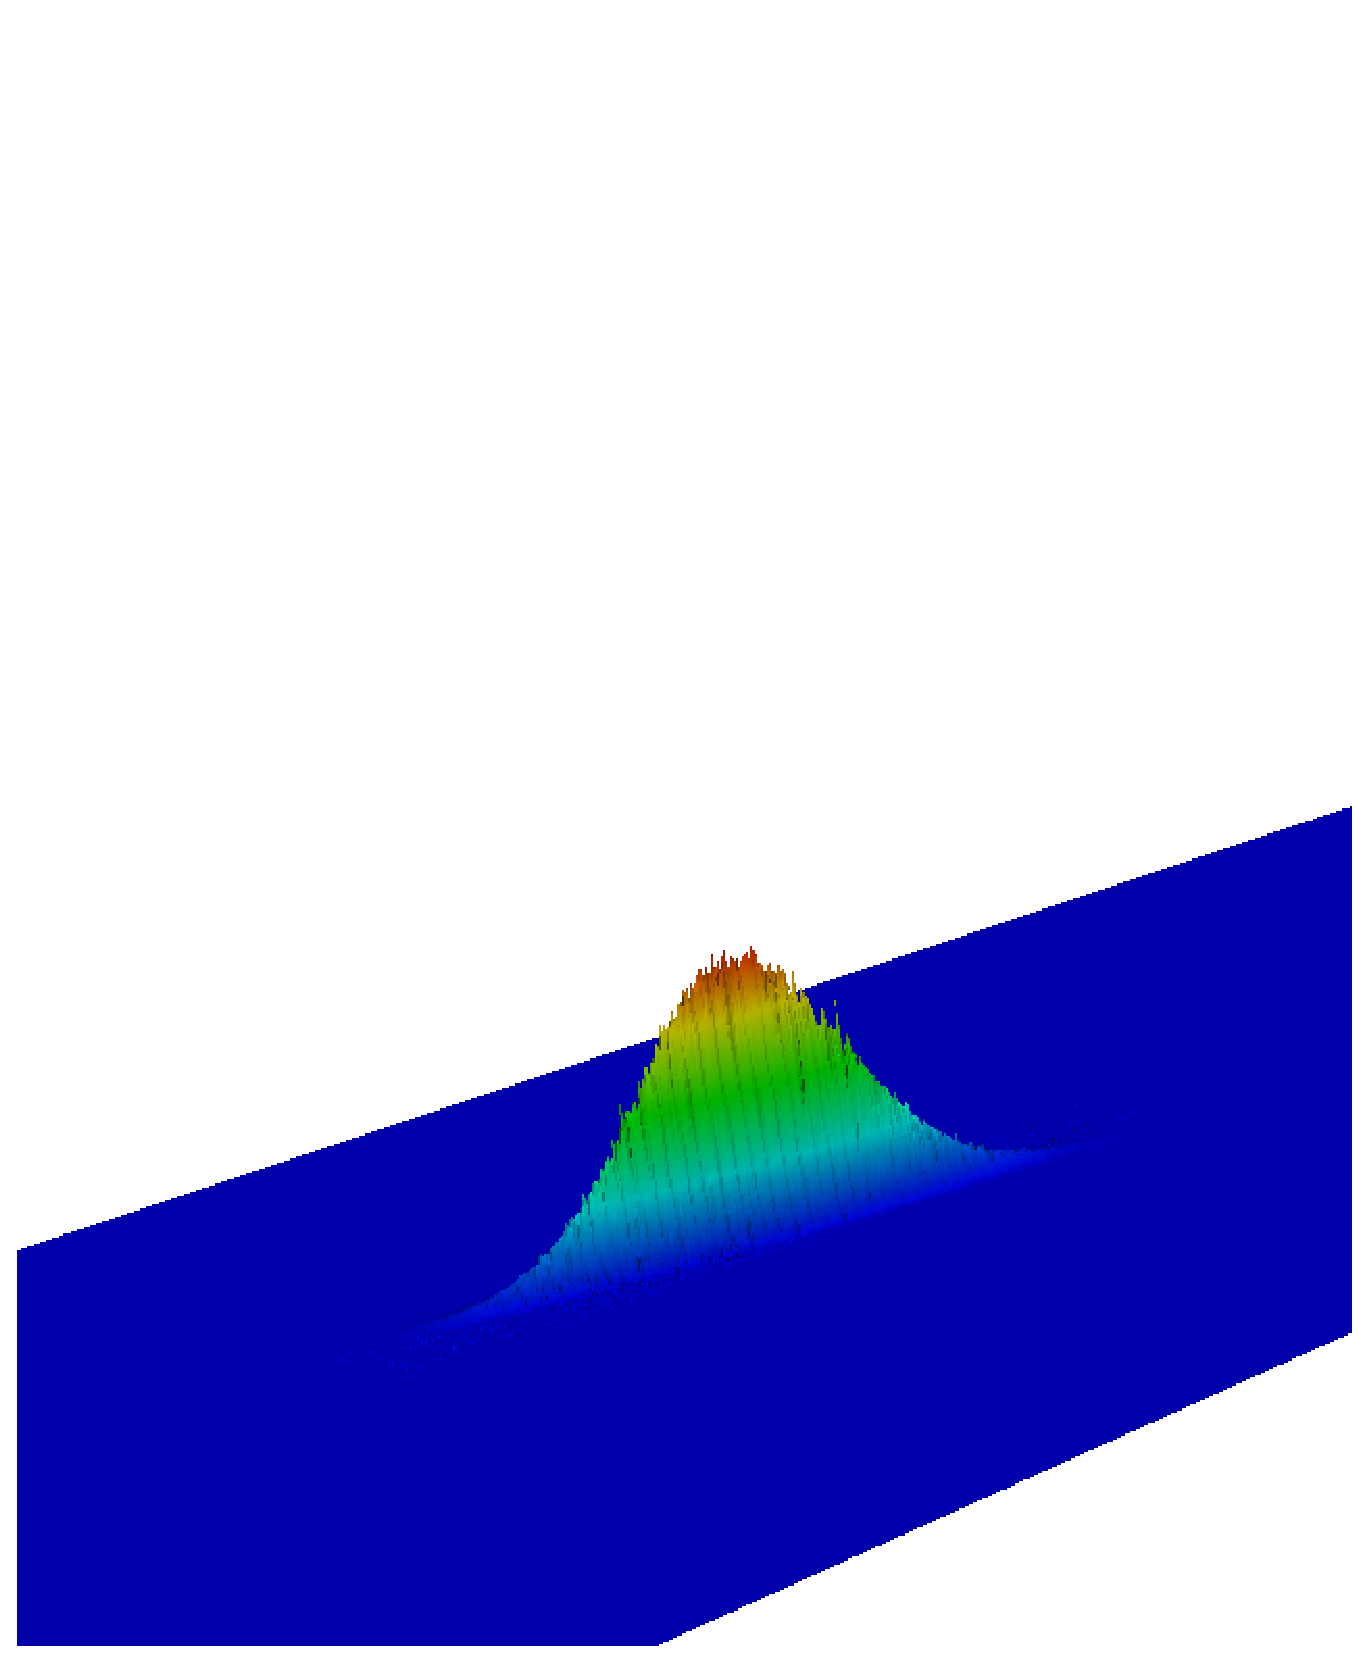
\includegraphics[width=0.5\columnwidth]{figures/wiens_prop1.eps}
  }
  \subfigure
  {
  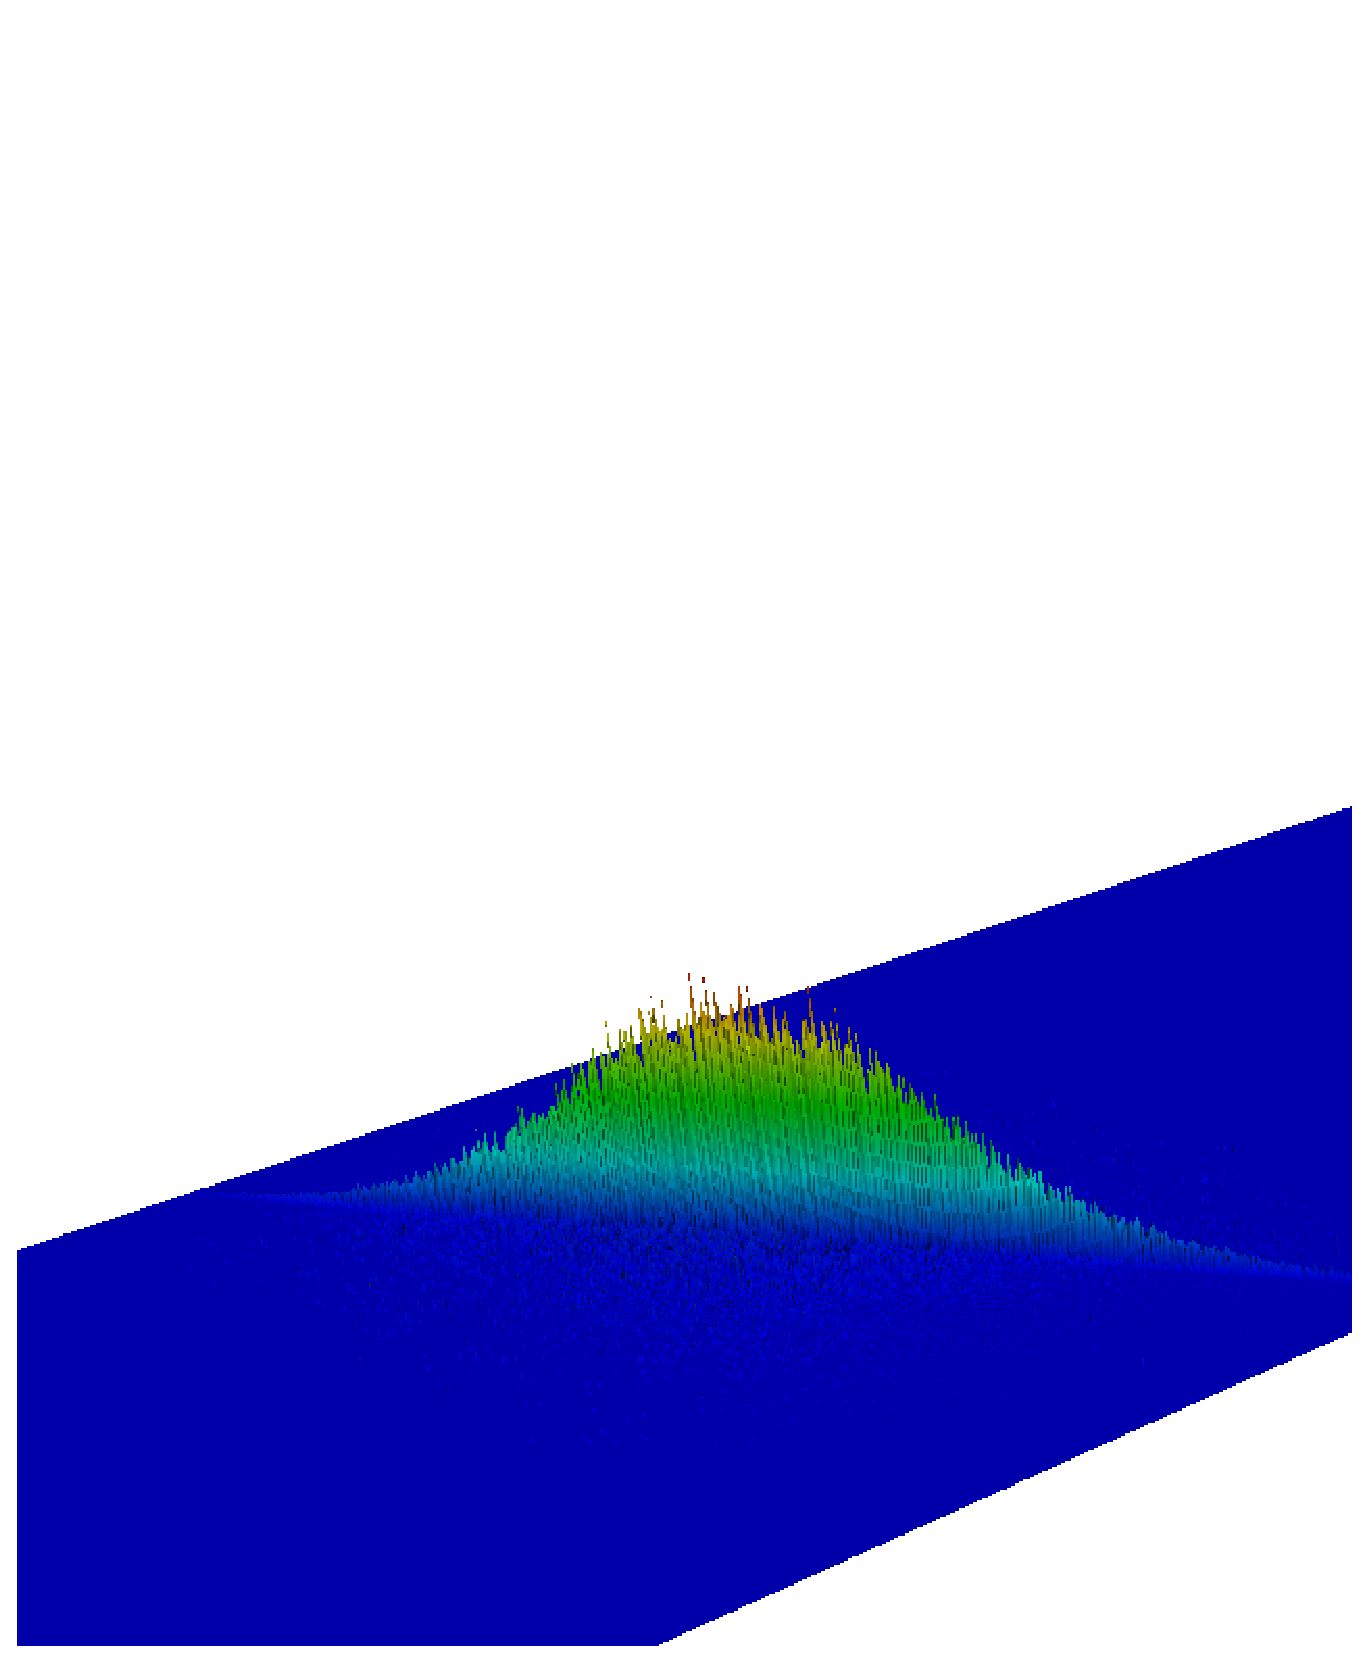
\includegraphics[width=0.5\columnwidth]{figures/wiens_prop9.eps}
  }
  \caption{
    Phase space distribution functions computed by the PD simulator are shown.
    In the classical case it can be interpreted directly
    as probability to find a particle, the indefinite nature in the
    quantum case, prohibits this direct interpretation, but still
    provides correct derived quantities such as density and momentum
    distribution. The evolution is shown at $100fs$ (\textbf{top})
    and at $1ps$ (\textbf{bottom}).
  }
  \label{fig:one}
\end{figure}

\clearpage

% ==============================================================================
% ==============================================================================
\section{Simulation Control} \label{wigner:sim}
% ==============================================================================
% ==============================================================================

The simulations are controlled via the input configuration and parameter XML files.
In the following the individual variables are explained in detail.

%\subsection{Parameters}



\begin{table}[ht!]
\centering
\begin{tabular}{|l|p{4.5cm}|c|c|}
\hline
\textbf{Variable}   & \textbf{Definition}   & \textbf{Unit} & \textbf{Default} \\
\hline
%\texttt{NI}  & FILLME & $m^{-3}$ & $1$ \\
%\hline
\texttt{TL}  & Lattice Temperature & $K$ & $300$ \\
\hline
%\texttt{Z}  &  FILLME  &  & $0.5e-12$ \\
%\hline
\texttt{effmass}  & Effective Mass Factor &  & $0.067$ \\
\hline
\texttt{alpha}  & Non-Parabolicity Factor & $1/eV$ & $0.61$ \\
\hline
\texttt{rho}  & Density & $kg/m^3$ &$5.36e3$ \\
\hline
%\texttt{us}  &  FILLME  & $m/s$ &$1./3. * ( 2. * 3.0e3  + 5.24e3 )$ \\
%\hline
%\texttt{DA}  &  FILLME  & $eV$ &$7.0$ \\
%\hline
%\texttt{energy\_beta}  &  FILLME  & $J$ &$1$ \\
%\hline
%\texttt{DO}  & FILLME   & $J/m$ &$1$ \\
%\hline
\texttt{optical\_phonon\_energy}  &  Optical Phonon Energy  & $eV$ &$0.0343$ \\
\hline
\texttt{polar\_optical\_phonon\_energy}  &  Polar Optical Phonon Energy  & $eV$ &$0.036$\\
\hline
\texttt{optical\_permitivity}  &  Optical Permitivity  & & $10.92$ \\
\hline
\texttt{static\_permitivity}  & Static Permitivity   & & $12.9$ \\
\hline
\texttt{free\_flight\_coeff}  &  Free Flight Coefficient  & $1/Hz$ & $1. / 2.6e13$ \\
\hline
\end{tabular}
\caption{The parameter variables are shown.}
\label{tab:paras}
\end{table}


%\subsection{Configuration}

%\clearpage

\begin{table}[ht!]
\centering
\begin{tabular}{|l|p{5cm}|c|c|}
\hline
\textbf{Variable}   & \textbf{Definition}   & \textbf{Unit} &\textbf{Default} \\
\hline
%\texttt{L}  &  FILLME   & m & 800 * 1e-9 \\
%\hline
%\texttt{p\_max}  &   FILLME  & 1/m & 6e-9 \\
%\hline
\texttt{x\_count}  & Number of simulation domain points in x-direction &  & 400 \\
\hline
\texttt{y\_count}  & Number of simulation domain points in y-direction &  & 3000 \\
\hline
\texttt{timestep}  & The time difference between two time steps &  s & 100.0e-15 \\
\hline
\texttt{max\_iterations}  & Number of simulated time steps &  & 10 \\
\hline
\texttt{max\_particle\_count}  &  Number of generated particles for each point in the phase space   &  & 30 \\
\hline
\end{tabular}
\caption{The configuration variables are shown.}
\label{tab:configs}
\end{table}

\clearpage

% ==============================================================================
\section{License}
% ==============================================================================

Boost Software License - Version 1.0 - August 17th, 2003

Permission is hereby granted, free of charge, to any person or organization
obtaining a copy of the software and accompanying documentation covered by
this license (the "Software") to use, reproduce, display, distribute,
execute, and transmit the Software, and to prepare derivative works of the
Software, and to permit third-parties to whom the Software is furnished to
do so, all subject to the following:

The copyright notices in the Software and this entire statement, including
the above license grant, this restriction and the following disclaimer,
must be included in all copies of the Software, in whole or in part, and
all derivative works of the Software, unless such copies or derivative
works are solely in the form of machine-executable object code generated by
a source language processor.

THE SOFTWARE IS PROVIDED "AS IS", WITHOUT WARRANTY OF ANY KIND, EXPRESS OR
IMPLIED, INCLUDING BUT NOT LIMITED TO THE WARRANTIES OF MERCHANTABILITY,
FITNESS FOR A PARTICULAR PURPOSE, TITLE AND NON-INFRINGEMENT. IN NO EVENT
SHALL THE COPYRIGHT HOLDERS OR ANYONE DISTRIBUTING THE SOFTWARE BE LIABLE
FOR ANY DAMAGES OR OTHER LIABILITY, WHETHER IN CONTRACT, TORT OR OTHERWISE,
ARISING FROM, OUT OF OR IN CONNECTION WITH THE SOFTWARE OR THE USE OR OTHER
DEALINGS IN THE SOFTWARE.



% ==============================================================================
% ==============================================================================
\chapter*{Appendix A}  \addcontentsline{toc}{chapter}{Appendix A: Visualization} \label{vis}
% ==============================================================================
% ==============================================================================
\section*{Visualization}
The majority of the generated outputfiles of the provided simulation tools utilize
the CSV format.
This CSV format is supported by various available tools, such as
the free open source tools ParaView ~\cite{paraview}, or Gnuplot~\cite{gnuplot} and the commercial MATLAB~\cite{matlab} suite.

In the following an exemplary visualization approach based on ParaView (Version 3.98.0) is depicted.
The first step of processing a CSV file is to load it via the \texttt{Open File} dialog.
As the the CSV output files generated by a ViennaWD simulator offer the \texttt{*.csv} file extension,
ParaView applies the corresponding file-processer automatically.
Fig.~\ref{fig:para1}-\ref{fig:para7} show the required steps. Several Paraview state files, containing predefined filter sequences, are included with the WEMC simulator under \texttt{wigner\_ensemble\_monte\_carlo/plot\_scripts} 

\begin{figure}[!ht]
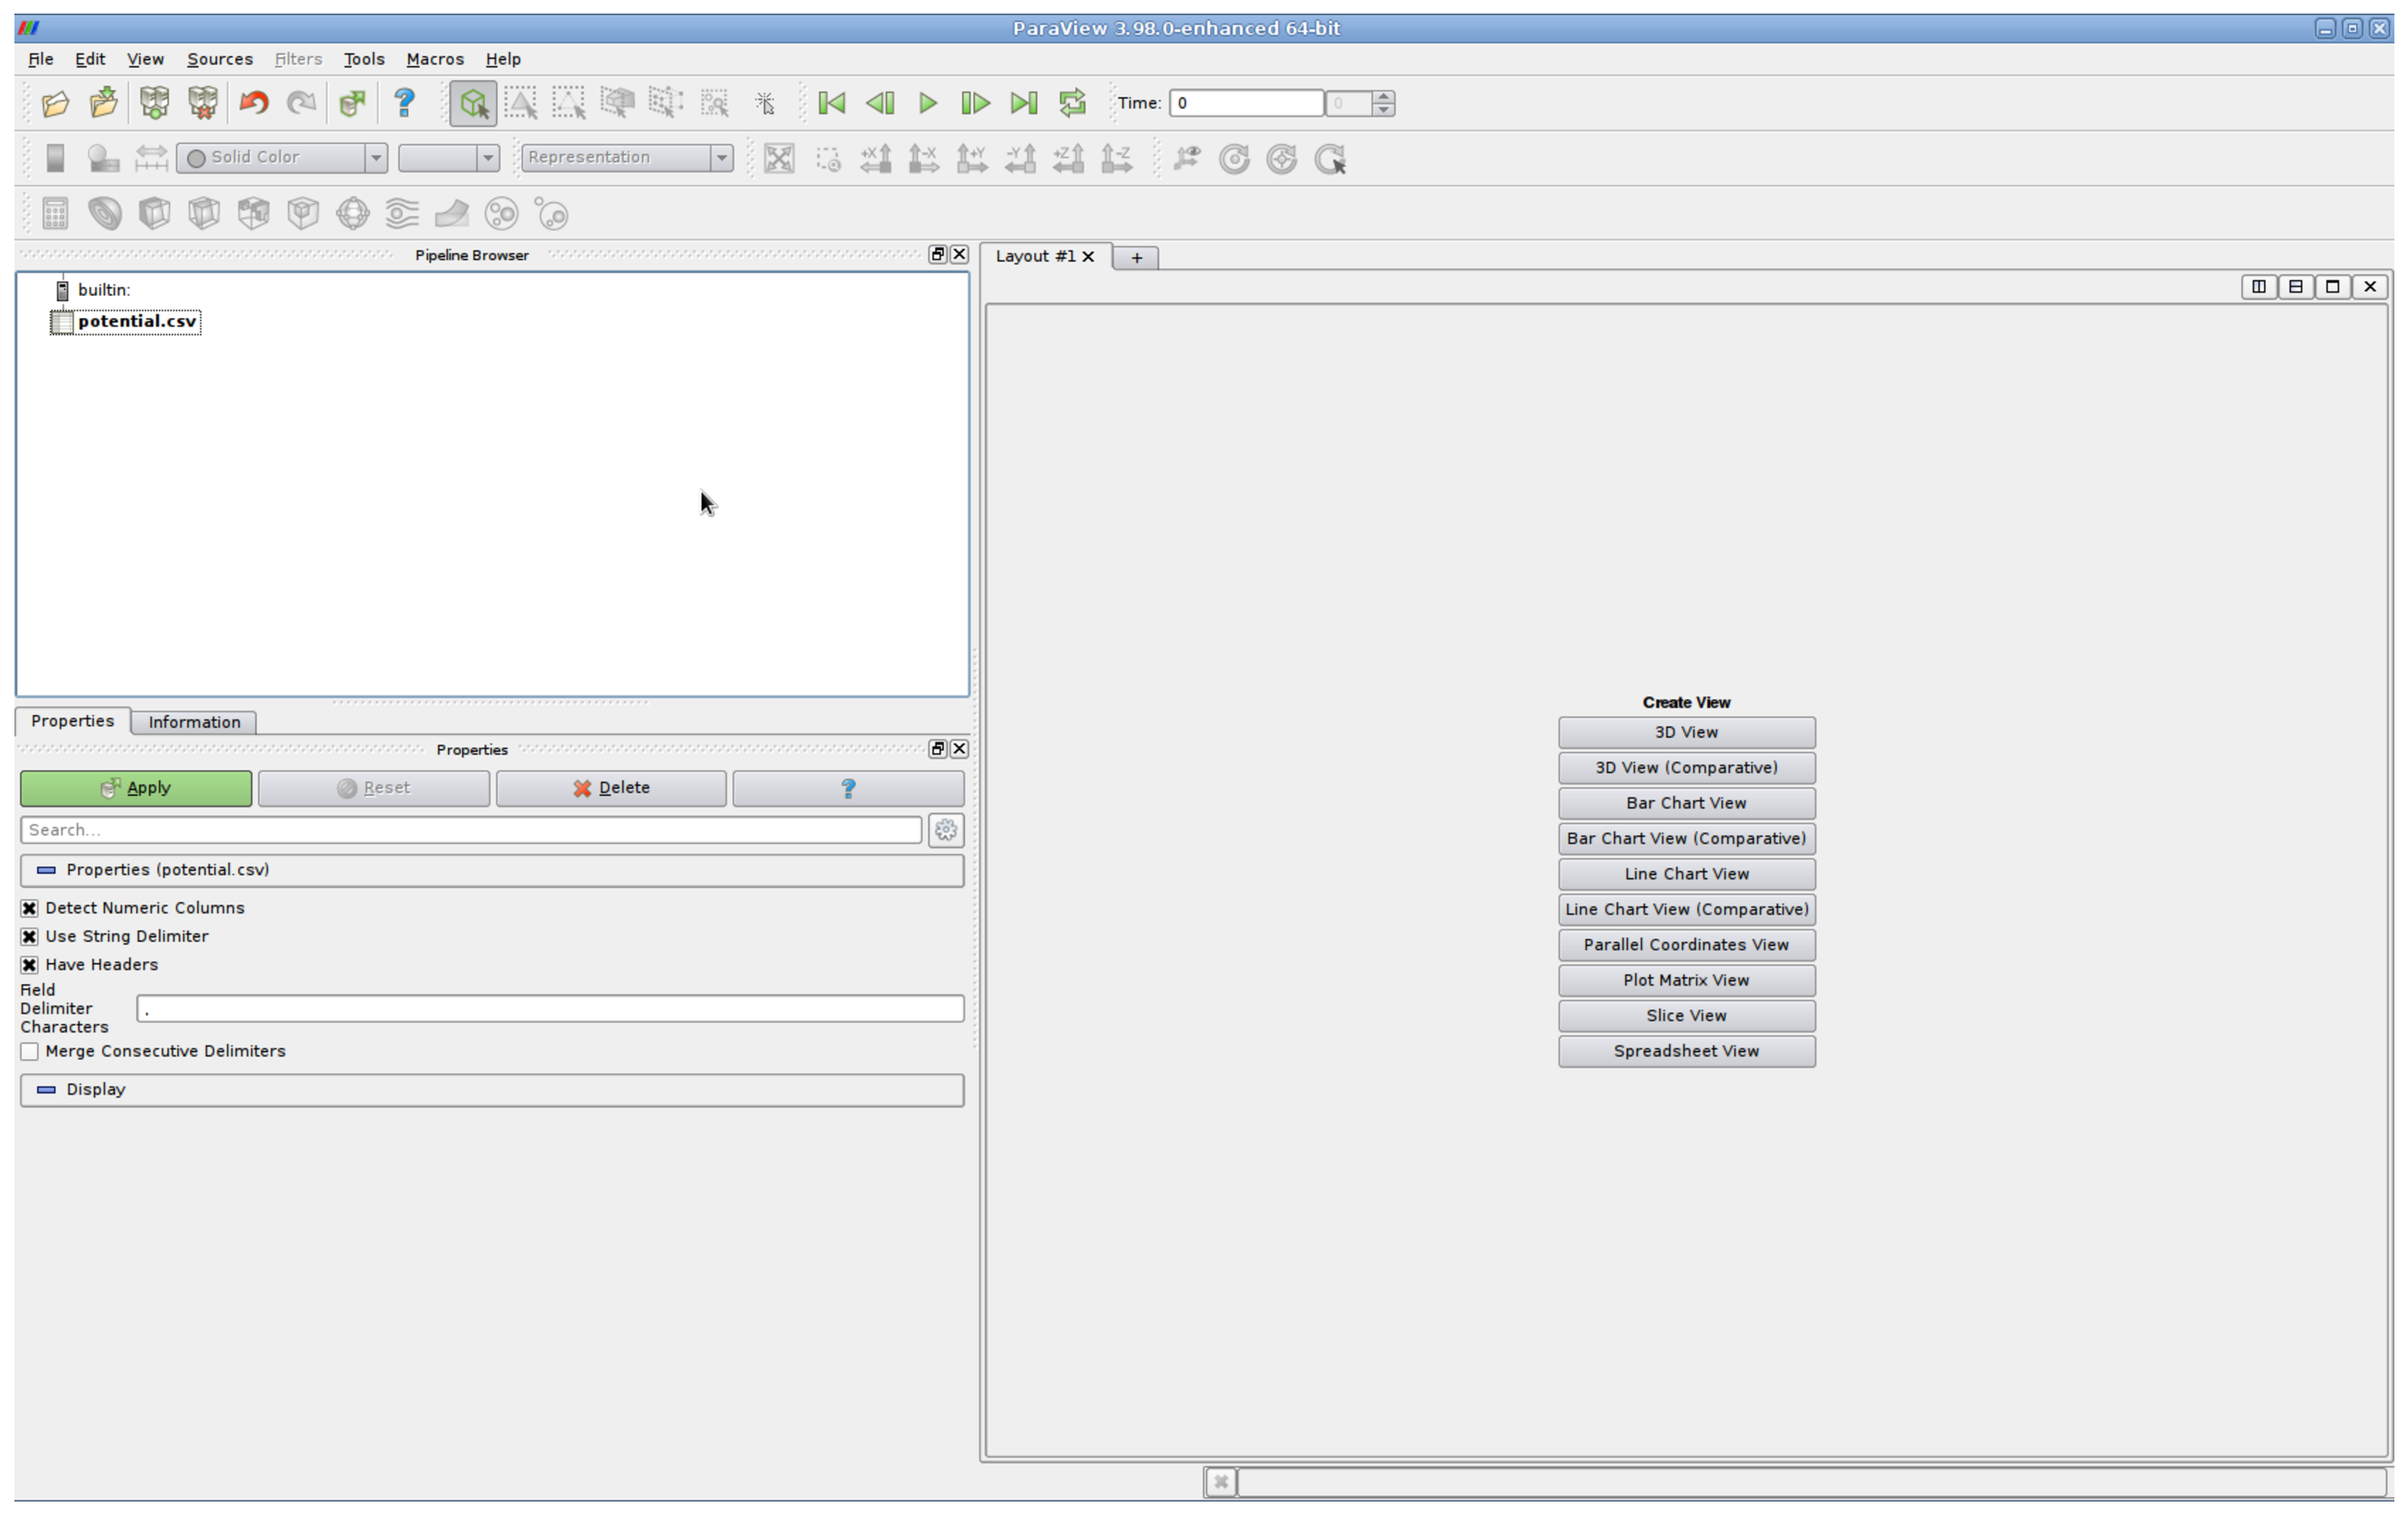
\includegraphics[width=1.0\columnwidth]{figures/para1.eps}
\caption{A CSV file has been loaded into ParaView.}
\label{fig:para1}
\end{figure}


\begin{figure}[!ht]
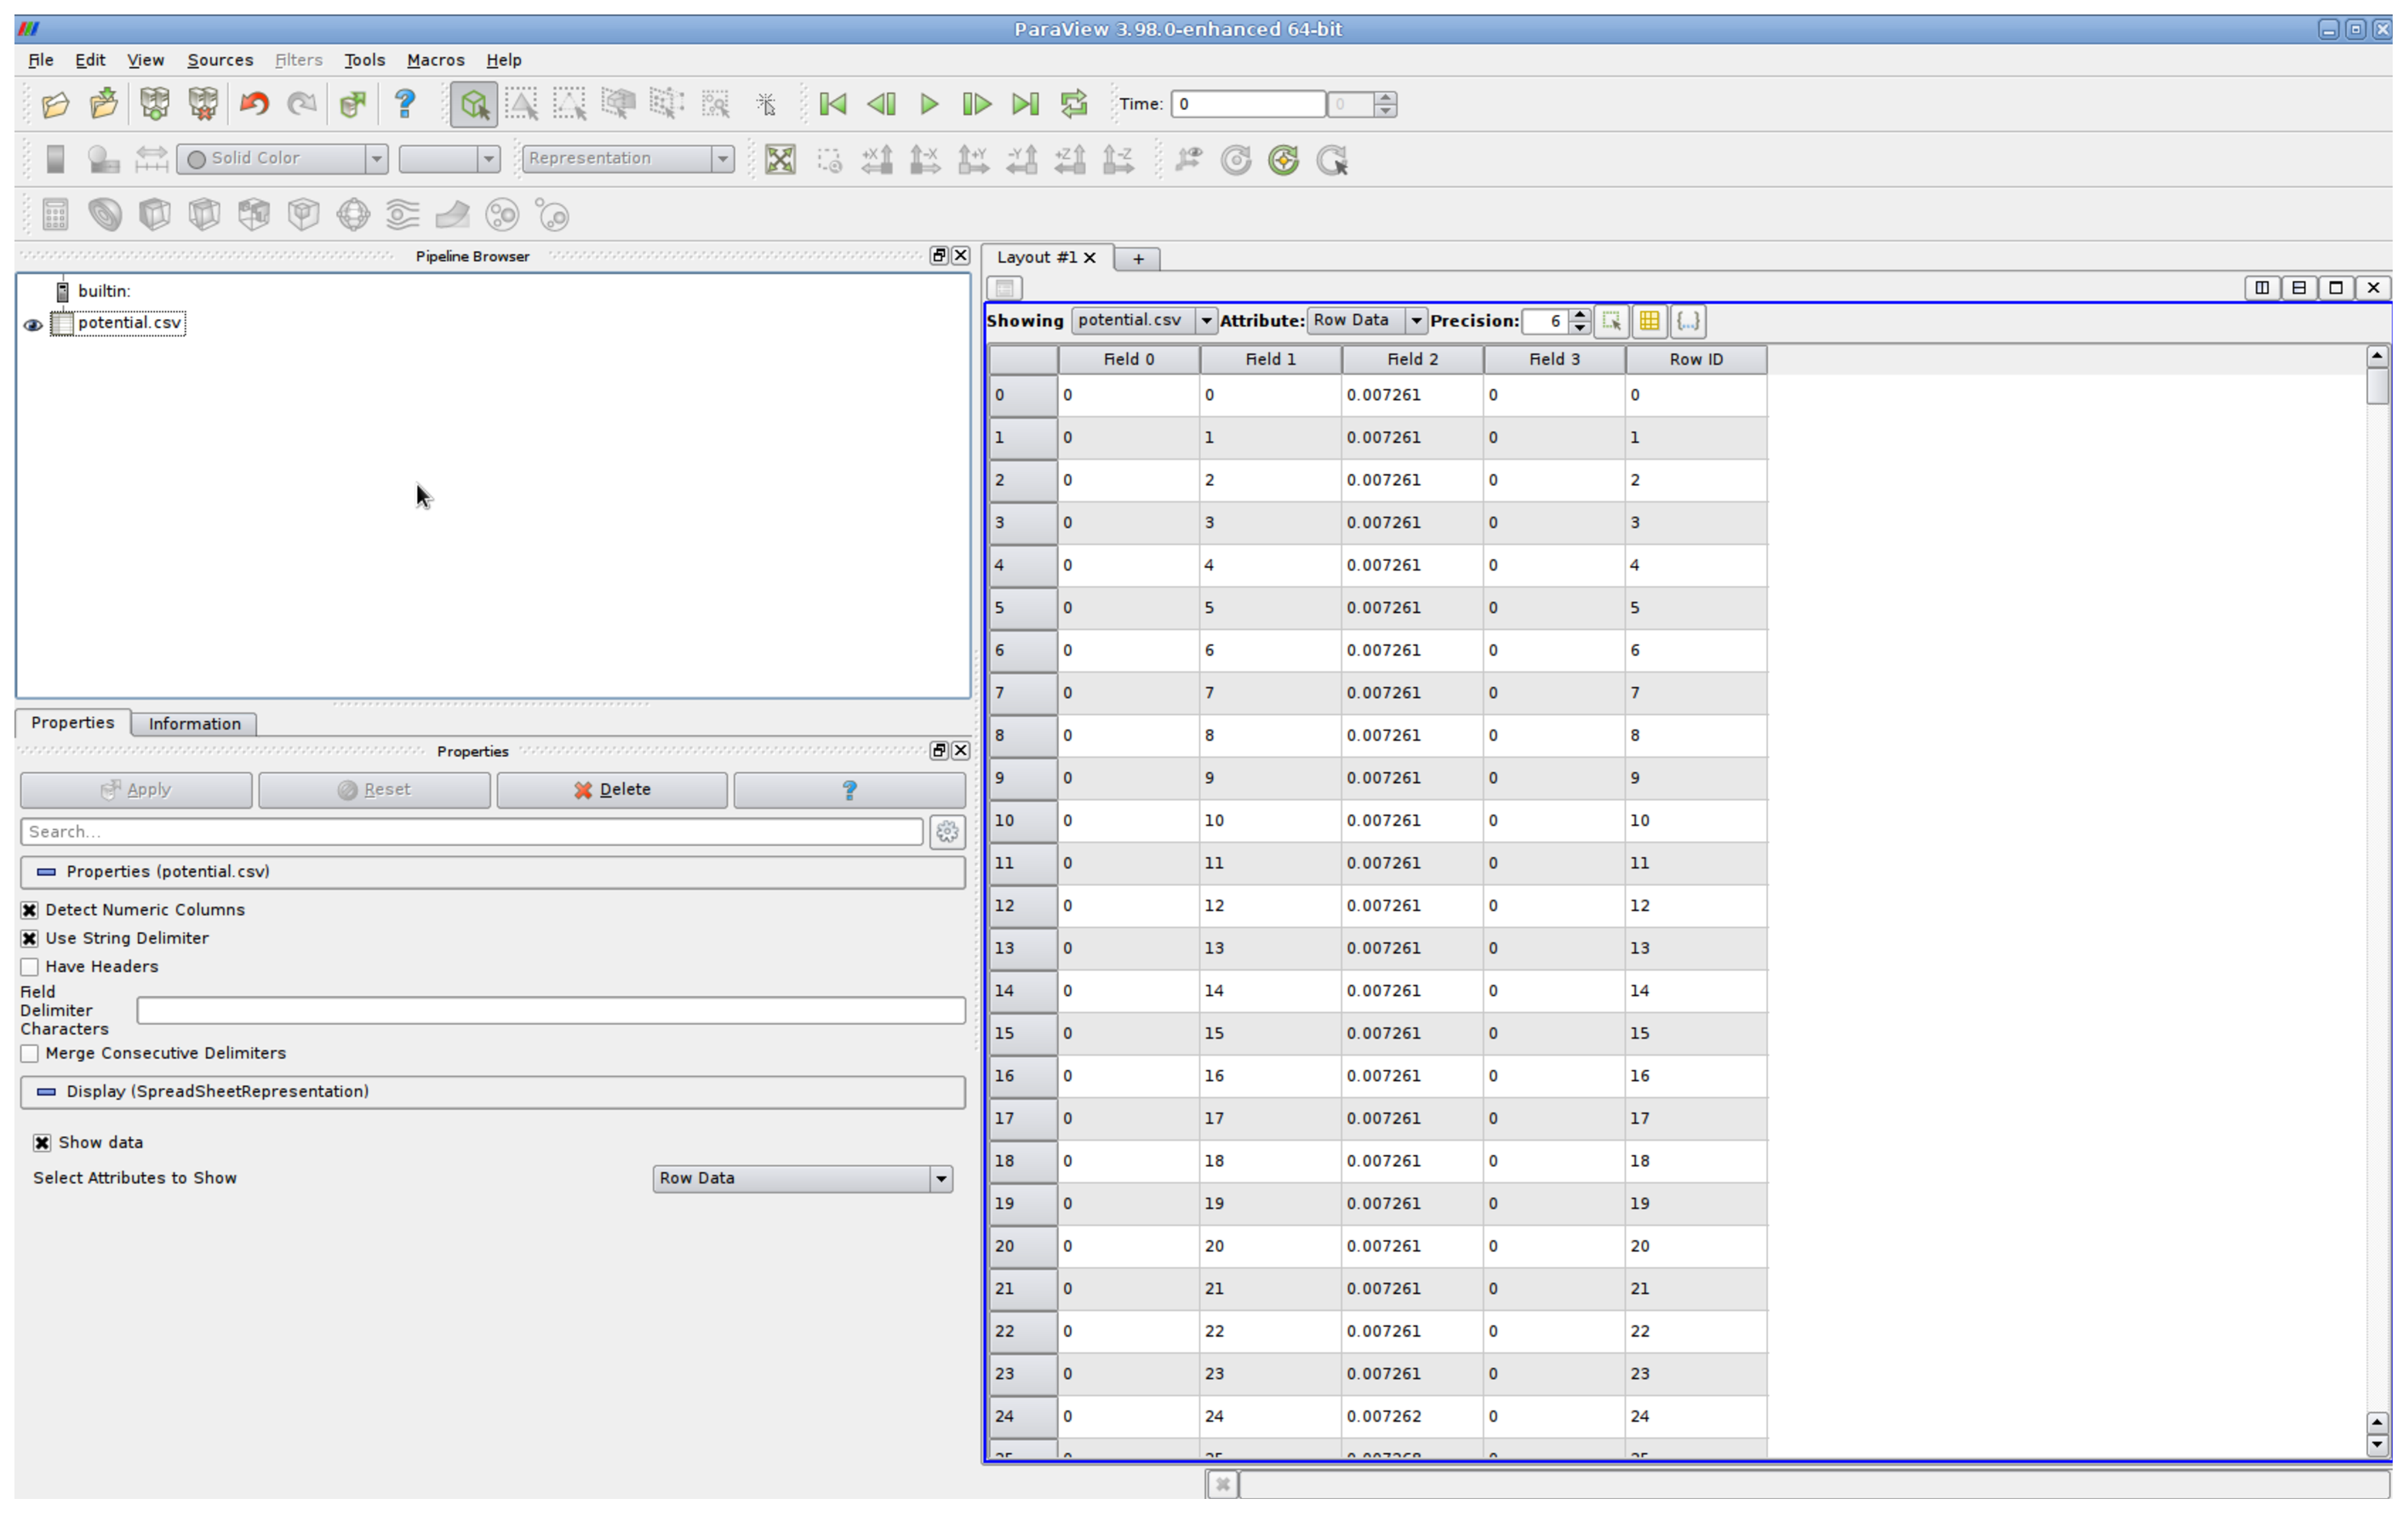
\includegraphics[width=0.9\columnwidth]{figures/para2.eps}
\caption{Headers are deactivated, as well as the comma has been replaced with a whitespace in the delimiter field.
After applying the changes, the table on the right is populated.}
\label{fig:para2}
\end{figure}

\begin{figure}[!ht]
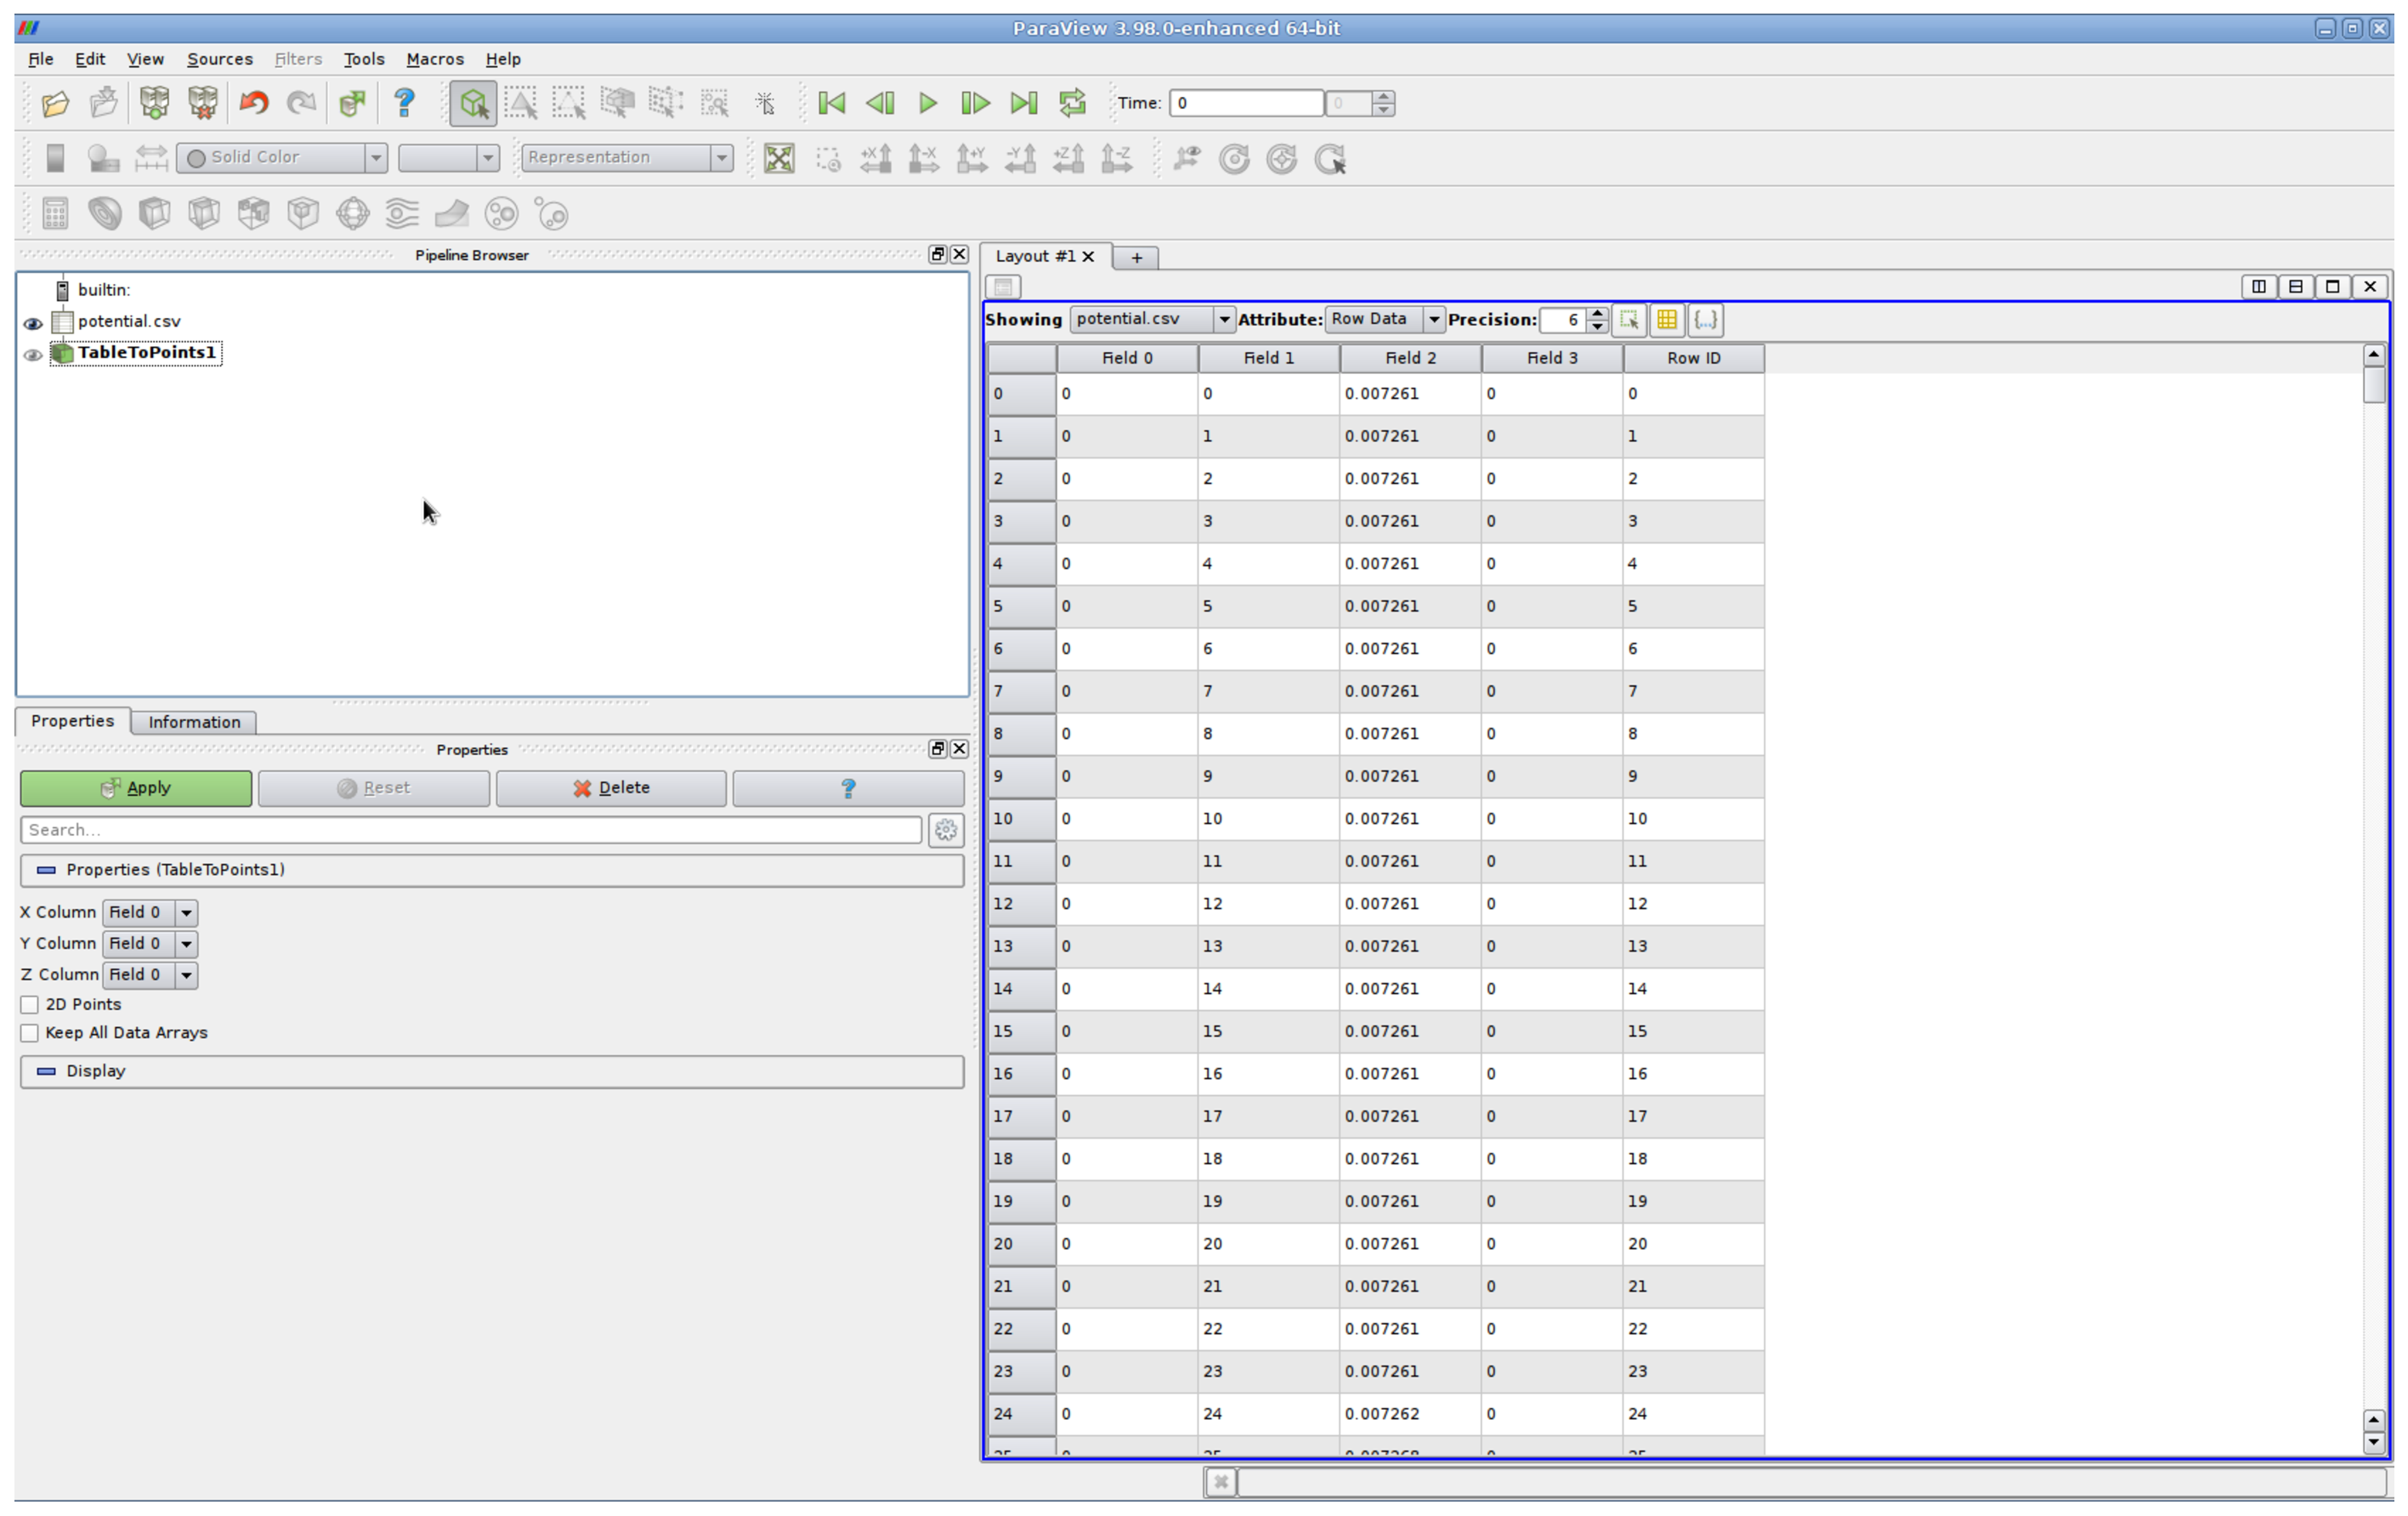
\includegraphics[width=0.9\columnwidth]{figures/para3.eps}
\caption{The \texttt{TableToPoints} filter has been added loaded.}
\label{fig:para3}
\end{figure}

\begin{figure}[!ht]
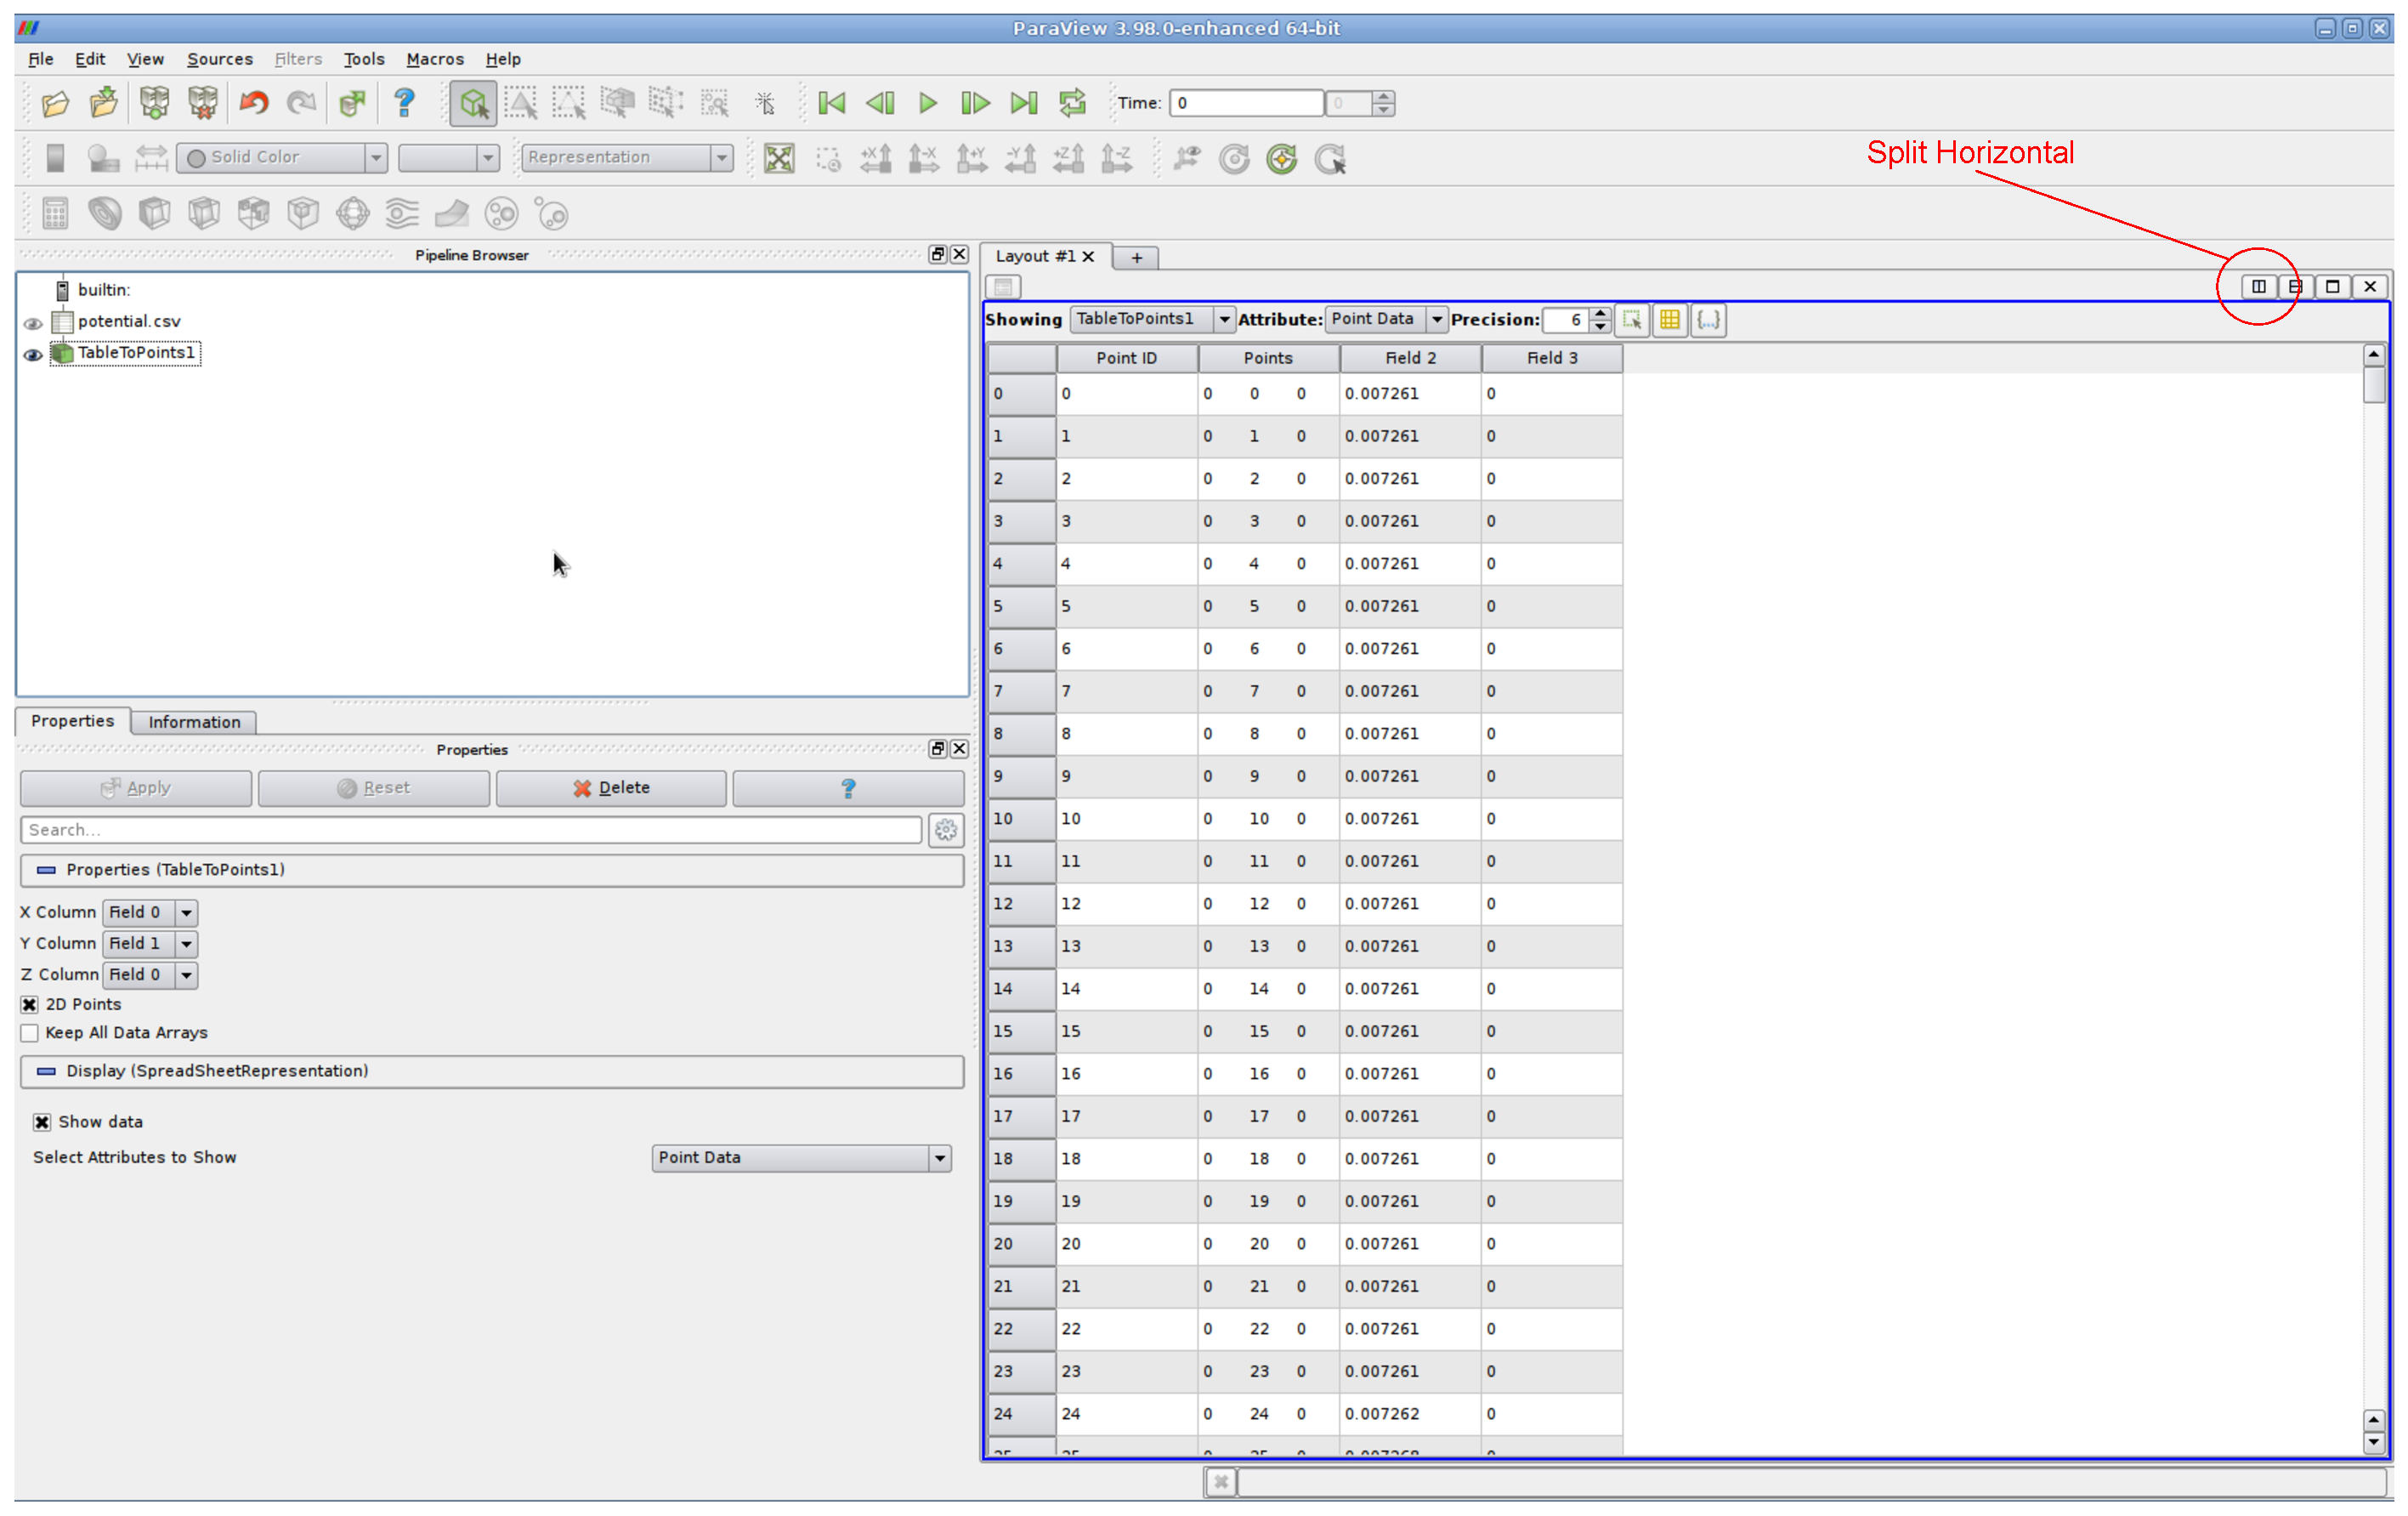
\includegraphics[width=0.9\columnwidth]{figures/para4.eps}
\caption{
The \texttt{TableToPoints} filter has been configured and applied.
Note that the X and Y column has been set to field 0 and 1, respectively.
Furthermore, the table is set to represent 2D data. Note that the Z column is therefore
obsolete.
A new 3D render view has to be created for visualizing the data in the subsequent steps.
This can be achieved, by pushing the \texttt{Split Horizontal} button.
}
\label{fig:para4}
\end{figure}

\begin{figure}[!ht]
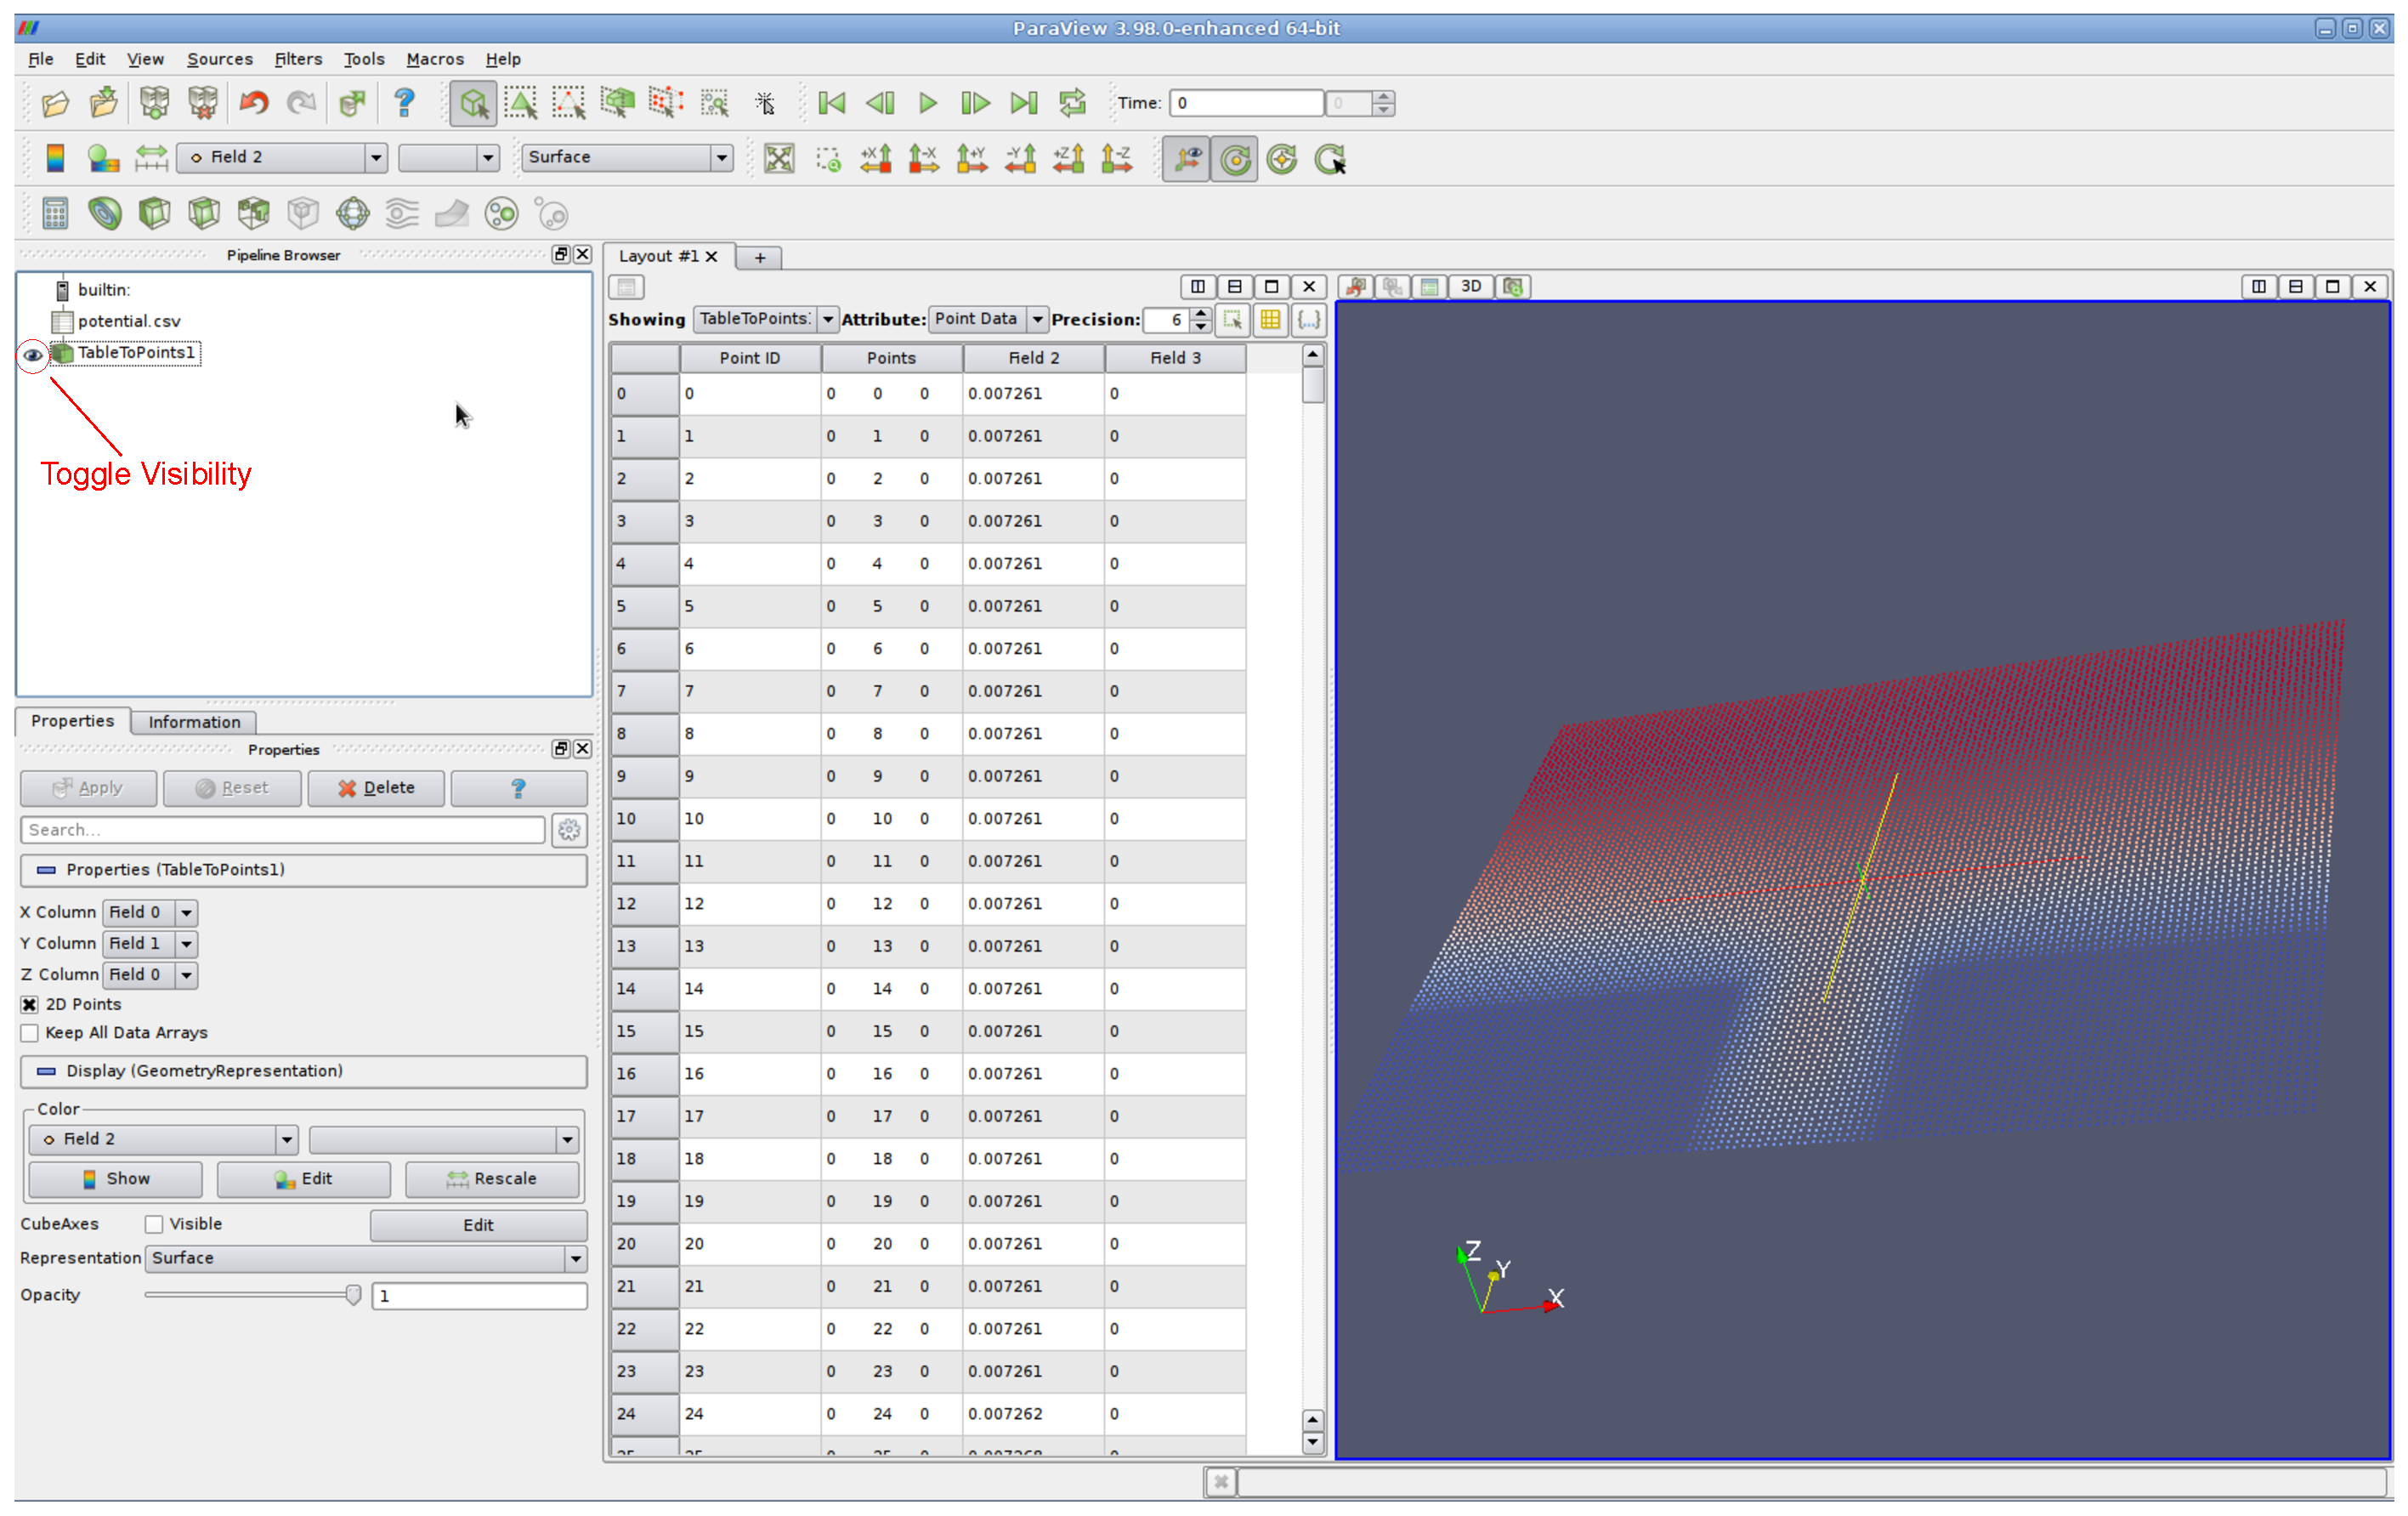
\includegraphics[width=0.9\columnwidth]{figures/para5.eps}
\caption{
The data can be actually visualized by activating the data via
hitting the 'greyed out eye' next to the \texttt{TableToPoints} filter on the left.
Coloring the output can be done by changeing from solid color to a data field, for instance, \texttt{Field 2}.
}
\label{fig:para5}
\end{figure}

\begin{figure}[!ht]
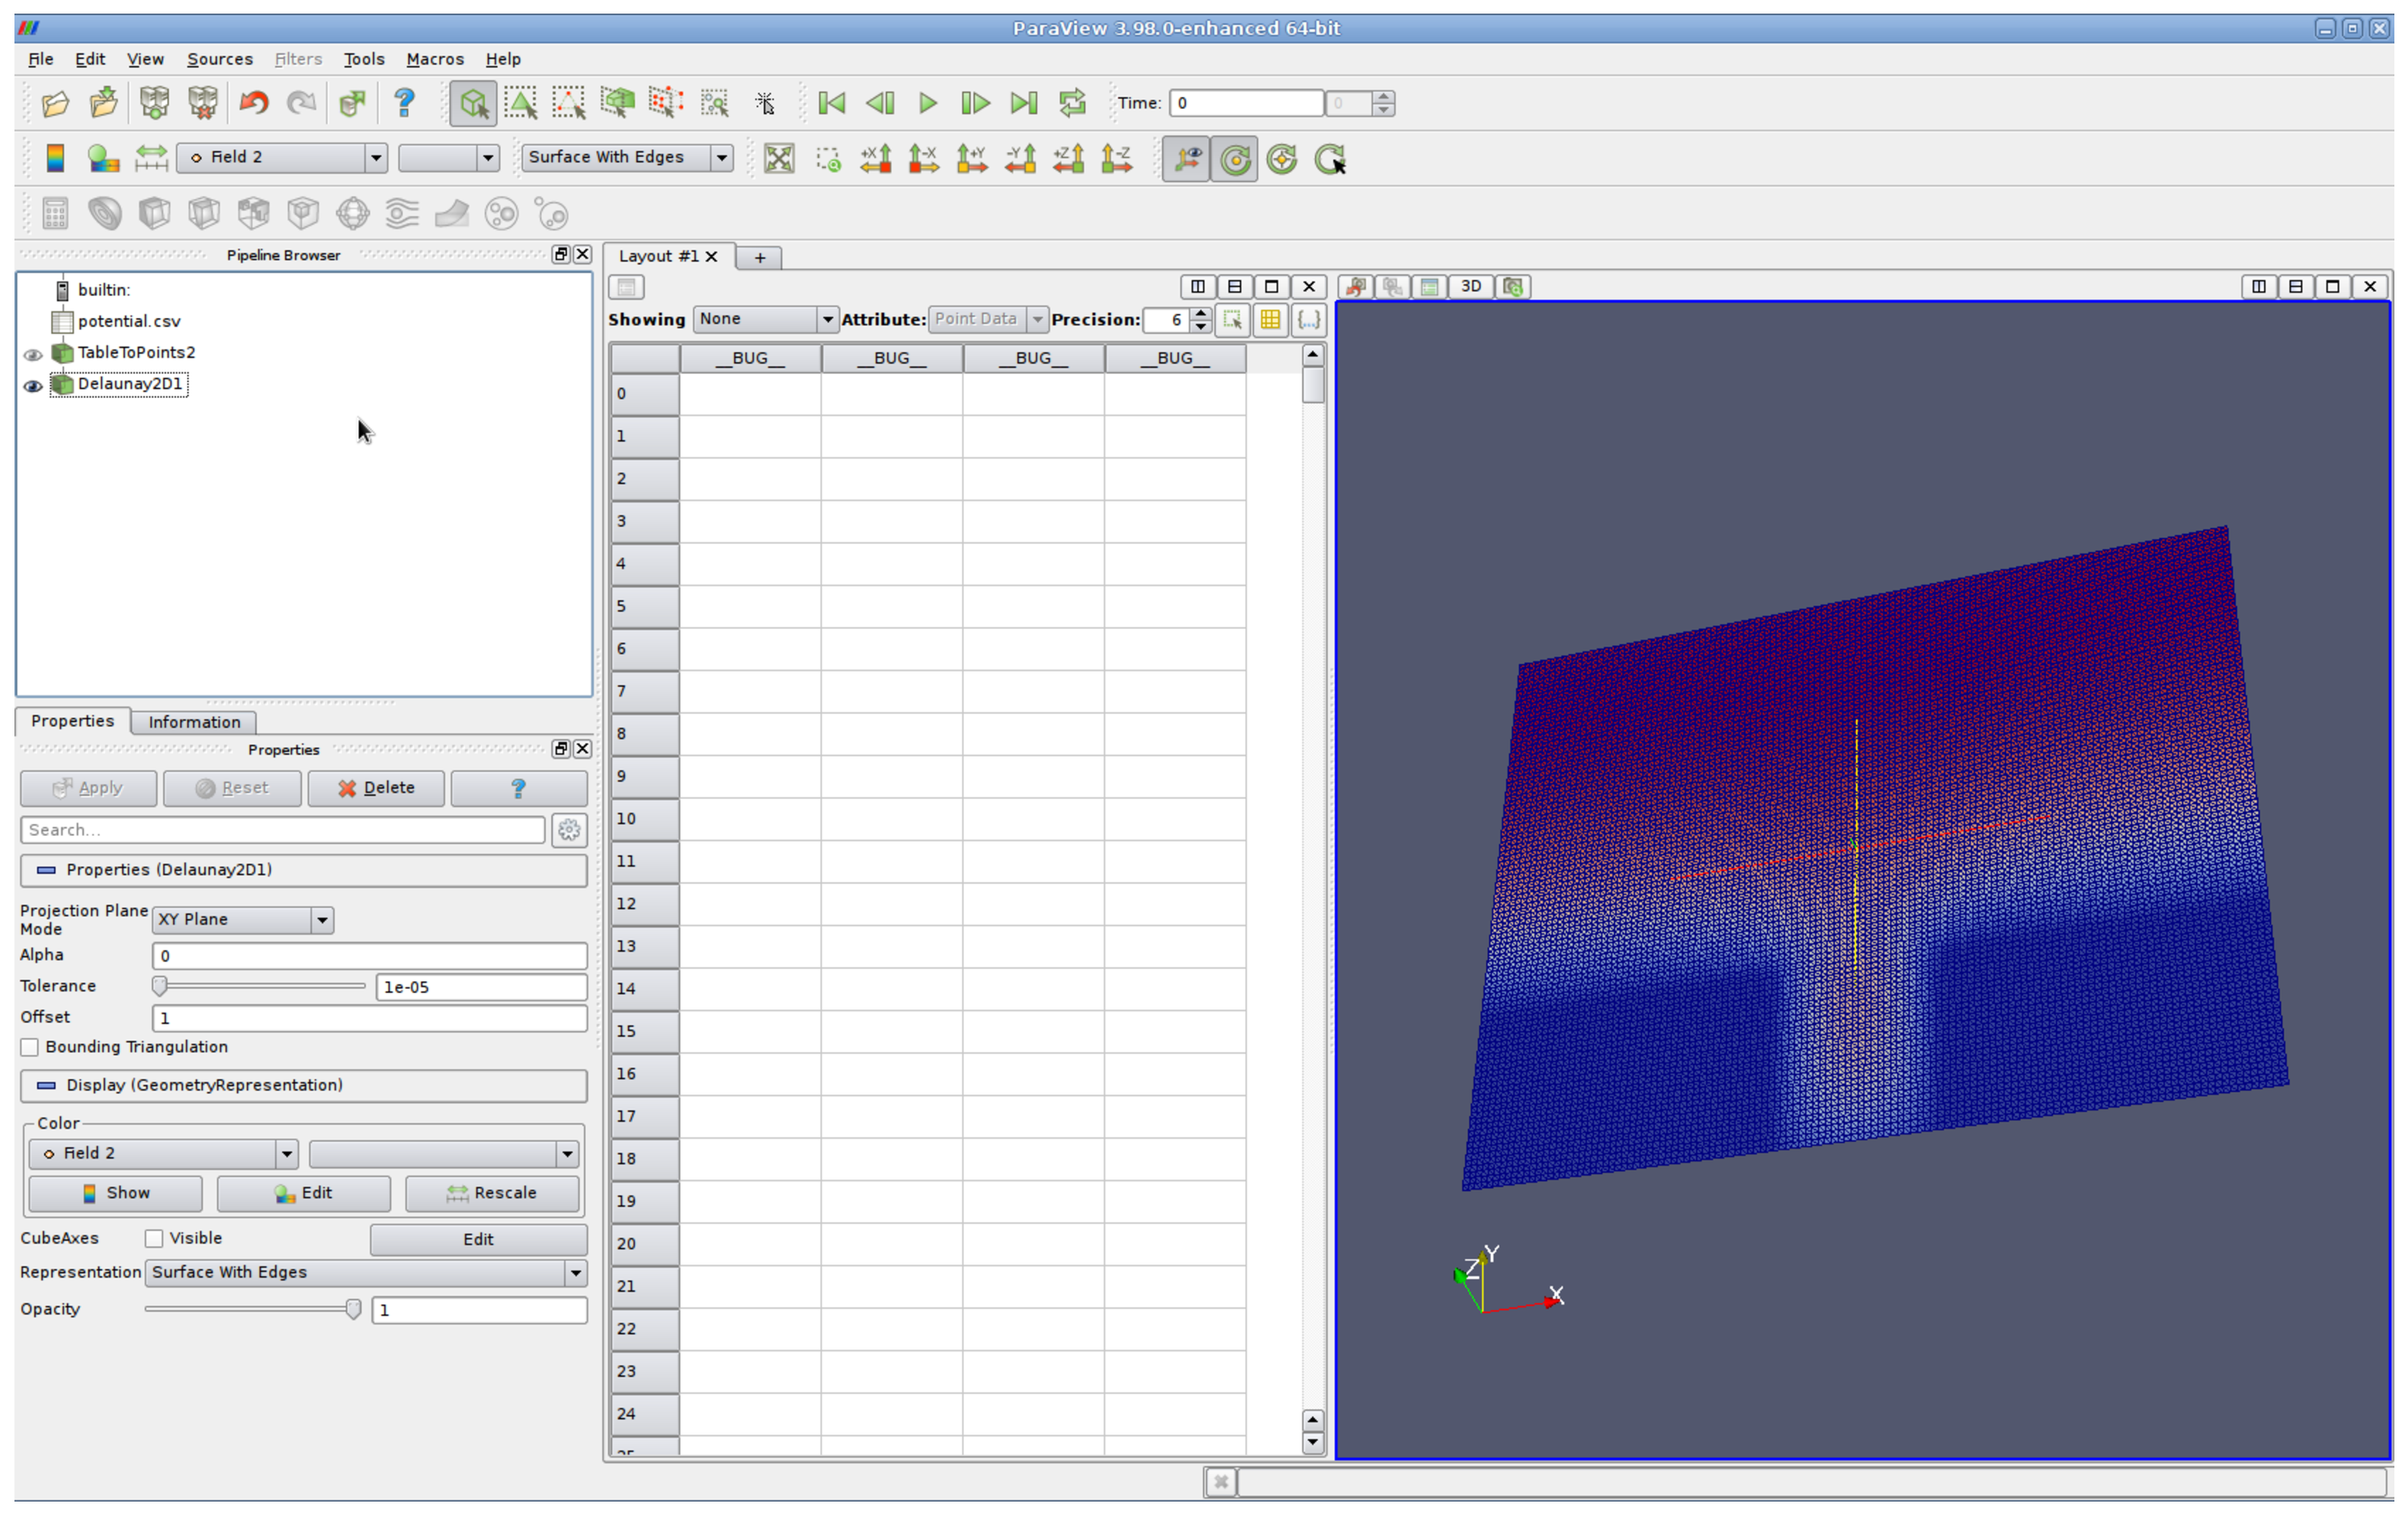
\includegraphics[width=0.9\columnwidth]{figures/para6.eps}
\caption{
So far only points have been visualized, similar to particles.
In case a mesh is required for visualization, the \texttt{Delaunay2D} filter can be used.
No configurations are required, simply adding and applying produces a 2D mesh.
}
\label{fig:para6}
\end{figure}

\begin{figure}[!ht]
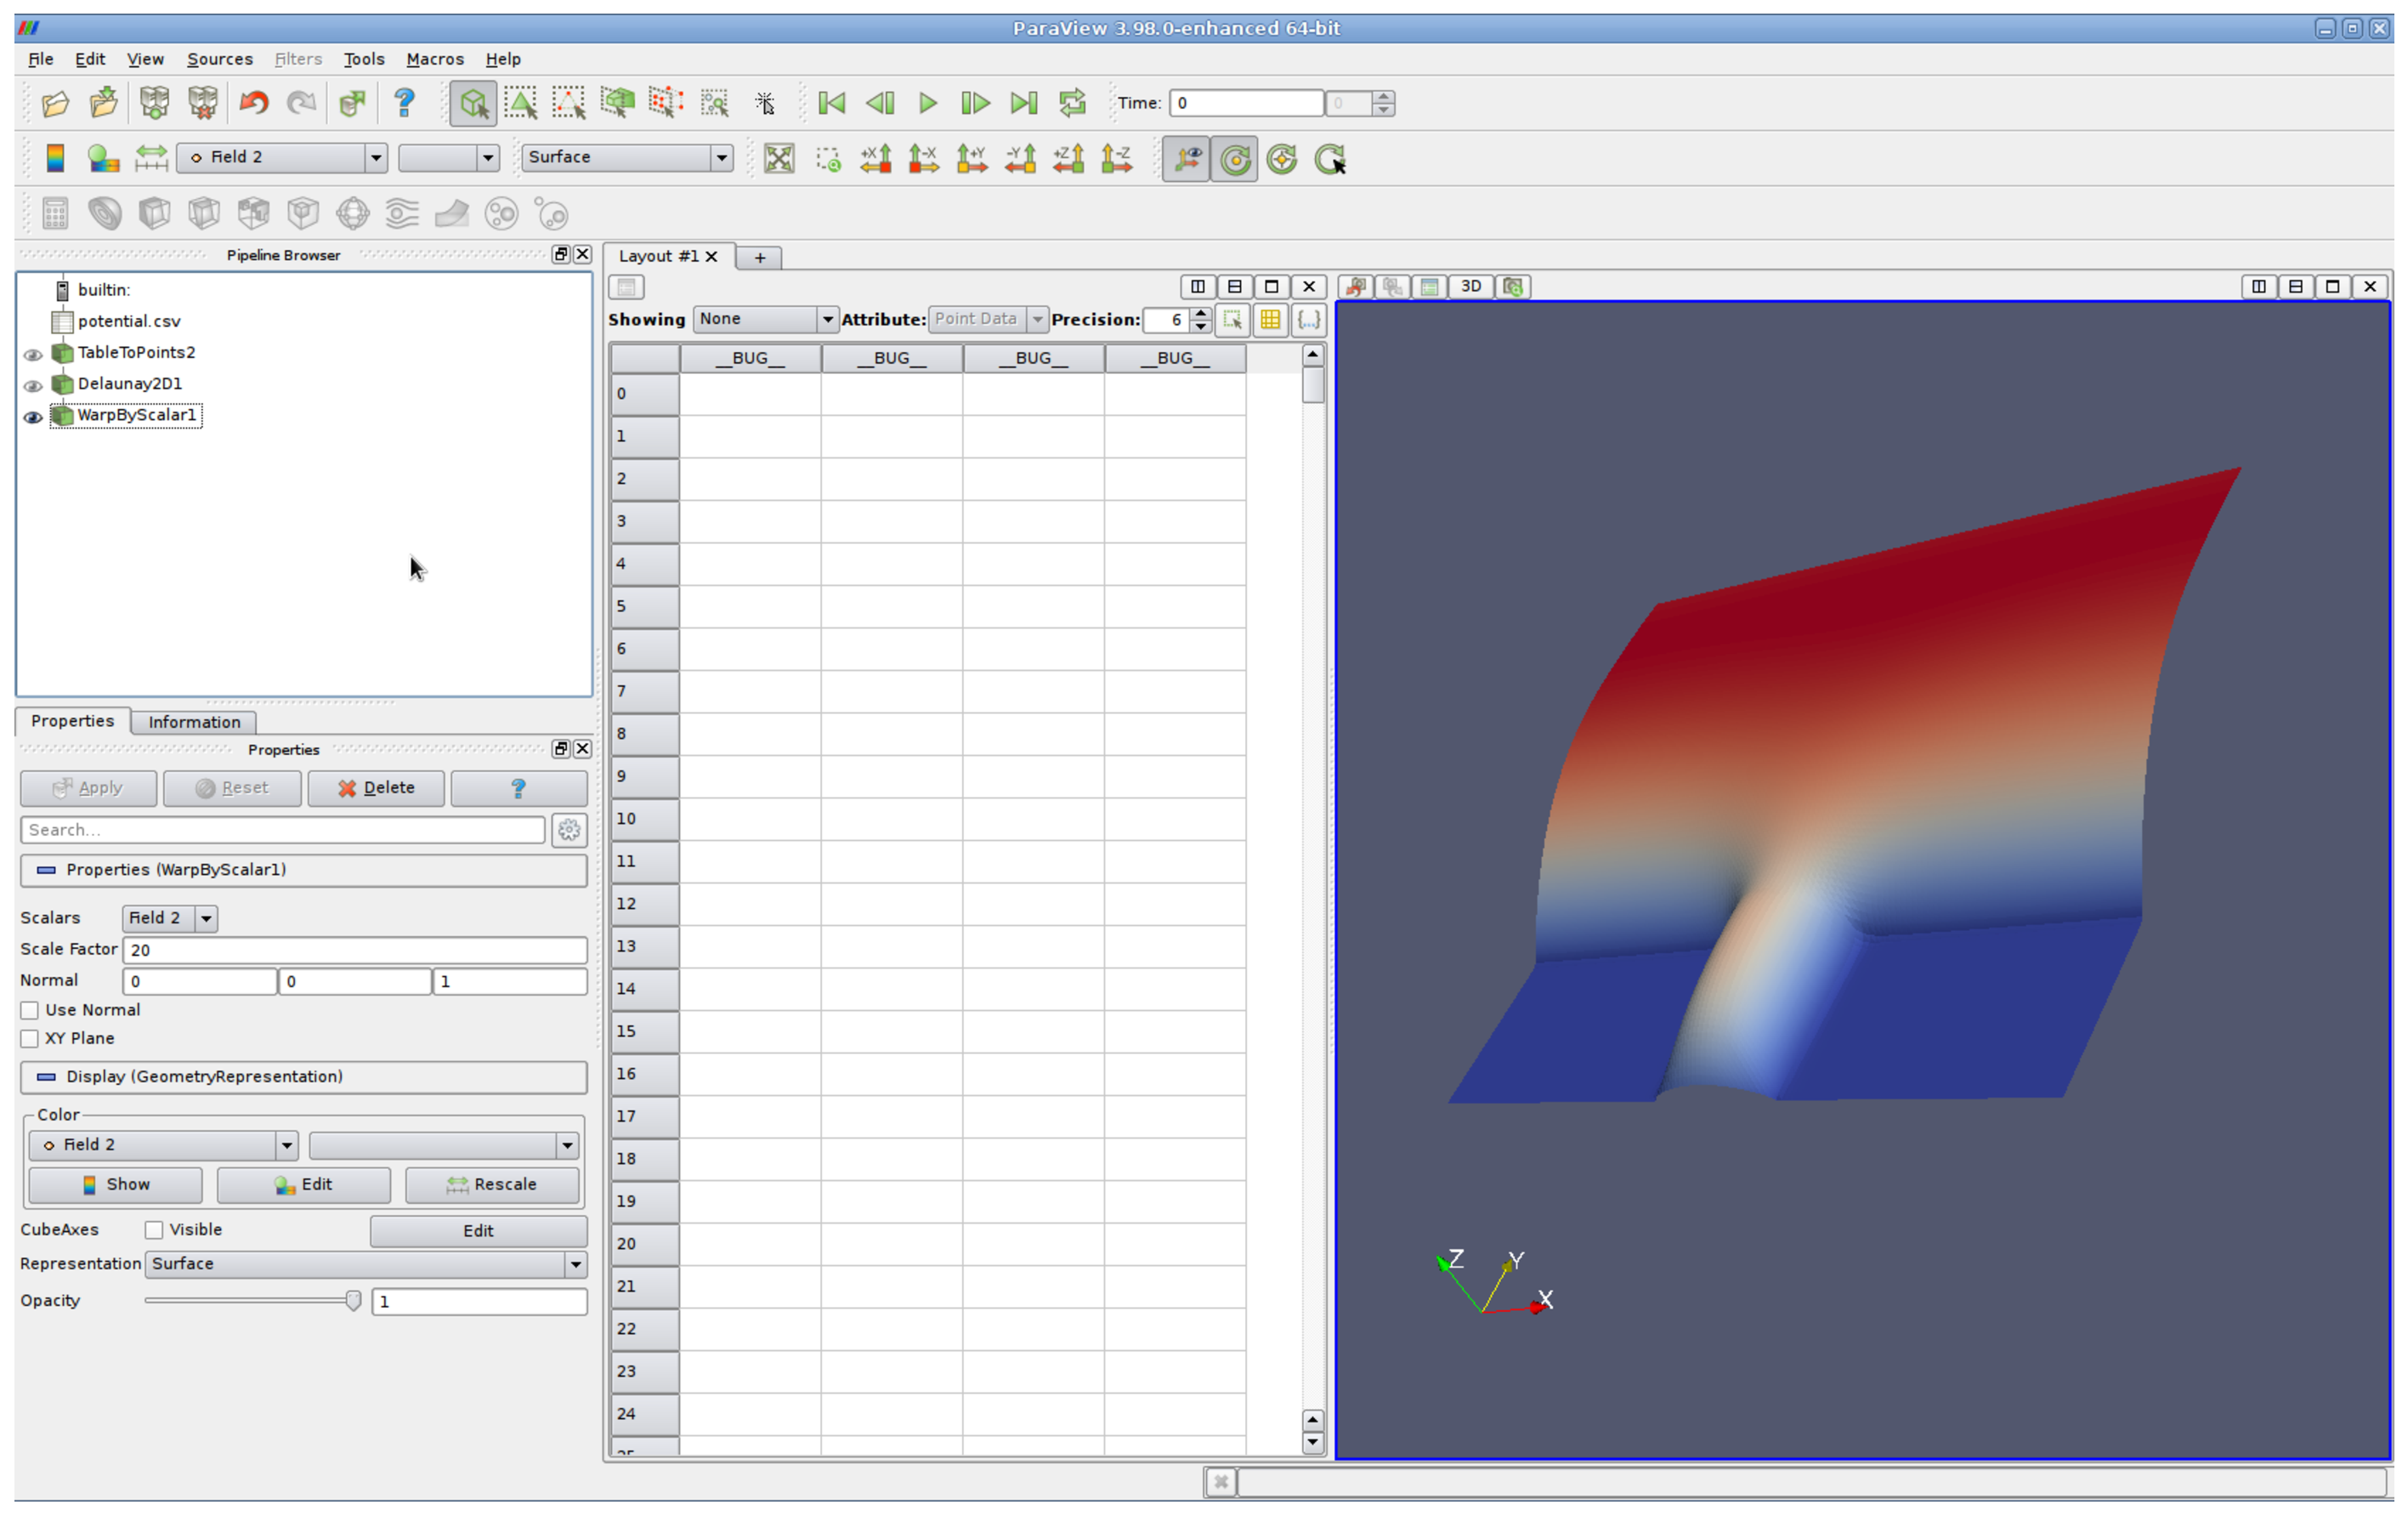
\includegraphics[width=0.9\columnwidth]{figures/para7.eps}
\caption{
For improving the visualization experience of 2D data, the quantity magnitude
can be correlated with a height or Z-coordinate. For this purpose, the \texttt{WarpByScalar} filter can be used.
By changeing the \texttt{Scale Factor} to a higher number, increased scaling is achieved.
}
\label{fig:para7}
\end{figure}

% ==============================================================================


\begingroup
\raggedright
%\bibliographystyle{IEEEtran_v1.13}
\bibliographystyle{MyIEEEtran}
\bibliography{literature}
\addcontentsline{toc}{chapter}{Bibliography}


\end{document}
